% !TeX encoding = UTF-8
% !TeX program = pdflatex
% !TeX spellcheck = it_IT
\documentclass[binding=0.6cm]{sapthesis}
\usepackage{microtype}
\usepackage[italian]{babel}
\usepackage[utf8]{inputenc}
\usepackage{hyperref}
\usepackage{listings}
\usepackage{biblatex}
\usepackage{graphicx}
%\graphicspath{{immagini/}}
\addbibresource{bibliografia.bib}
%\lstset{basicstyle=\ttfamily, breaklines=true}
\usepackage{xcolor}  % Pacchetto per la gestione dei colori
\usepackage{caption}
\usepackage{amsmath}
\usepackage{amssymb}

\captionsetup{font=it}  % Imposta il font delle didascalie in corsivo


% Impostazioni di base per lstlisting
\lstset{
    basicstyle=\ttfamily,  % Usa un font monospace per il codice
    backgroundcolor=\color{gray!10},  % Sfondo leggermente grigio
    frame=single,  % Aggiunge un bordo attorno al codice
    %caption={didascalia},  % Didascalia del blocco di codice
    captionpos=b,  % Posizione della didascalia (b = bottom, t = top)
    escapeinside={(*@}{@*)},  % Permette di aggiungere LaTeX all'interno del codice se necessario
}
\renewcommand{\lstlistingname}{Codice}


\hypersetup{pdftitle={La mia tesi},pdfauthor={Francesco Biccari}}
\title{Generazione e visualizzazione grafica di traffico di reti}
\author{Francesco Pannozzo}
\IDnumber{699427}
\course{Laurea Triennale in Informatica}
\courseorganizer{Facoltà di Ingegneria dell'Informazione, Informatica e Statistica}
\AcademicYear{2023/2024}
\advisor{Prof. Daniele De Sensi}
\authoremail{francesco.pannozzo@libero.it}
\copyyear{2024}
\thesistype{Relazione di tirocinio}
\begin{document}
\frontmatter
\maketitle
\dedication{Dedicato alla\\ mia famiglia}
\begin{abstract}
Questa relazione descrive il lavoro di tirocinio interno svolto presso l'università La Sapienza, 
concretizzato nella realizzazione 
di un progetto volto a realizzare un software per poter visualizzare in forma grafica l'andamento 
del traffico di una rete.
Il progetto ha come obiettivo di mostrare il traffico di rete al variare del tempo e ciò viene raggiunto
tramite grafiche e animazioni generate programmaticamente. L'idea dell'ambito di tirocinio nasce 
dalla volontà di sperimentare una realizzazione front-end tramite la libreria Manim, un motore di animazioni per video
matematici esplicativi. Nel capitolo dedicato all'introduzione descriveremo l'ambito in cui si è tenuto il tirocinio, le motivazioni
alla base in cui è stato idealizzato l'argomento, seguito da un'analisi dello stato dell'arte attuale, descrivendo diverse realtà affini al progetto
e studiandone caratteristiche, i loro pregi e mancanze. A seguire ci sarà una descrizione dei contributi che vuole dare il progetto, scaturiti dall'analisi
dello stato dell'arte e infine una breve panoramica sulla base di partenza del progetto, descrivendo da cosa si è partiti, come è nata l'argomentazione
che ha portato alla scelta del progetto e la modalità di svolgimento. Nel capitolo 2 parleremo del contesto di sviluppo, ovvero le tecnologie impiegate.
Seguirà quindi una descrizione approfondita della scelta di certe tecnologie ma soprattutto del perchè le si è scelte. Il capitolo 3
descriverà il generatore di traffico e configurazione di rete, descrivendone funzionalità, condizioni inziali di setup di questa parte di applicazione e infine
descrivendo come il tutto viene generato, passando dalla distribuzione spaziale dei nodi e creazione dei links all'ottenimento dei files sui quali sono memorizzati i dati ottenuti.
Il capitolo 4 tratterà l'analizzatore di traffico, nello specifico dell'implementazione della logica che risiede dietro l'analisi del file contenente il traffico.
Il capitolo 5 sarà sul visualizzatore grafico, in cui verrà fornita una manoramica sulle logiche dietro la creazione degli elementi grafici e delle animazioni, le modalità
grafiche che è possibile ottenere, la descrizione delle scelte di design legate all'aspetto grafico e una sezione dedicata all'accessibilità, con cui si tratterà
l'implementazione di soluzioni che trattano il tema del daltonismo. Il capitolo 6 darà un quadro generale sulla complessità computazionle delle sezioni di codice più sensibili, analizzando gli andamenti asintotici di tutte le principali parti.
Infine avremo il capitolo 7, in cui tireremo le conclusioni del progetto.

\end{abstract}
\tableofcontents
\mainmatter
\chapter{Introduzione}
Nel mondo le reti informatiche sono oramai un concetto ben istanziato 
nella colletività, la loro presenza è soverchiante e si dirama nei più disparati settori.
Basti pensare già alle  reti PAN (Personal Area Network) le quali connettono dispositivi
personali entro pochi metri e che ognuno di noi usa abitualmente nella propria casa, 
alle reti LAN (Local Area Network), 
anch'esse presenti
nelle nostre case così come in uffici o edifici scolastici, le reti dei data center 
fino a giungere alla rete globale internet, la quale è creatrice a sua volta di paradigmi come
può essere l'internet of things. Le reti informatiche sono impiegate nei più vari 
settori come l'istruzione, in cui le reti
sono cruciali nelle scuole e nelle università per avere accesso a risorse educative o sfruttare l'e-learning, i servizi
pubblici governativi e sanitari, nel settore ludico e multimediale come il gioco online e l'attuale
streaming di contenuti multimediali: insomma, le reti informatiche sono di fatto una presenza piena e diffusissima
ed è estremamente difficile riuscire a immaginare il mondo come lo vediamo oggi senza questa tecnologia.
Con l'aumentare delle funzionalità legate alle reti, così come i dispositivi collegati a esse, capire cosa succede al
loro interno, come si muovono i dati, è quindi di cruciale importanza, tramite l'analisi dei dati che vi fruiscono è possibile fare diagnostica, per quanto
riguarda un discorso di monitoraggio, ma è anche possibile applicare le analisi in un ambito didattico e accademico.
Capire cosa sta succedendo in una rete in modo immediato e visivo è lo scopo di questo progetto, il quale punta a mostrare,
in modo grafico, l'andamento del traffico di una rete.
\section{Ambito del tirocinio}
Il progetto fa parte del percorso di tirocinio interno intrapreso presso l'Università La Sapienza di Roma. L'argomento su cui verte il progetto
è la realizzazione di un visualizzatore grafico dell'andamento del traffico di una rete, basato
su animazioni programmatiche. Il tool permette di visualizzare gli switch rappresentanti 
i vari endpoints e i link
che li collegano i quali vengono colorati tramite animazioni nel tempo in base al traffico di 
rete precedentemente analizzato. Nel tool è presente anche una parte generativa di traffico di rete,
una creazione di traffico fittizia di vitale importanza ai fini di testing. Il progetto è suddiviso quindi in tre parti; una parte
che si occupa della generazione di una configurazione network e relativo traffico di rete, 
una parte che analizza il traffico di rete
calcolandone le medie percentuali di intervalli di tempo e aggiornate ripetutamente e infine 
una parte che visualizza il traffico analizzato
dall'analizzatore producendo una rappresentazione video.
\section{Motivazioni}
L'idea di sviluppare un visualizzatore grafico di traffico di rete è nata, 
in sede di proposta, dal Professore Daniele De Sensi, relatore del tirocinio, e dalla mia volontà di sviluppare un'applicazione avente il front-end
come focus dell'esperienza. Nel mio personale corso di studi presso il Dipartimento di Informatica non ho avuto modo
di studiare e approfondire un discorso legato al front-end, per cui la volontà di intraprendere questo percorso
nasce in primis da un forte interesse verso questo aspetto dell'informatica e in secondo luogo per un completamento di formazione professionale personale.
\section{Stato dell'arte}
\label{sec:stato_arte}
L'esigenza di analisi di reti informatiche ha portato alla luce svariati tool che permettono
appunto di analizzare cosa avviene in una rete, di studiarne i dati statistici e di visualizzare
graficamente determinati scenari. L'universita americana Johns Hopkins\cite{JohnsHopkinsUniversity2024} ha stilato una lista
di software per la visualizzazione e analisi di reti\cite{JHUDatavisNetwork2024}:




\begin{itemize}
  \item \textbf{Gephi\cite{Gephi2024}:}
  Gephi è il software leader di visualizzazione ed esplorazione per tutti i tipi di grafici e reti ed è open source. Le sue caratteristiche includono
  l'analisi esplorativa dei dati mediante manipolazioni di reti in tempo reale, 
  analisi dei collegamenti per rivelare le strutture sottostanti delle associazioni tra oggetti, 
  analisi dei social network per la creazione di connettori di dati sociali per mappare le organizzazioni della comunità e le reti di piccoli mondi, 
  analisi della rete biologica per rappresentazione di modelli di dati biologici ed esportazione e 
  creazione poster per promuovere e divulgare il lavoro scientifico con mappe stampabili di alta qualità.
  \item \textbf{Cytoscape\cite{Cytoscape2024}:} è una piattaforma software open source per visualizzare 
  reti complesse e integrarle con qualsiasi tipo di dati. Consiste in una piattaforma per
  visualizzare reti di interazioni molecolari e percorsi biologici, potendo integrare queste reti con annotazioni,
  profili di espressione genica e altri dati. Originariamente progettato per la ricerca biologica, 
  ora è una piattaforma generale per l'analisi e la visualizzazione di reti complesse.
  \item \textbf{GraphVis\cite{Graphviz2024}:} è un software di visualizzazione di grafici open source. Caratteristiche,
  I programmi di layout Graphviz accettano descrizioni di grafici in un semplice linguaggio di testo e creano diagrammi in formati utili, 
  come immagini e SVG per pagine web; PDF o Postscript per l'inclusione in altri documenti; 
  o visualizzare in un browser grafico interattivo. Graphviz ha molte funzionalità utili 
  per diagrammi concreti, come opzioni per colori, caratteri, layout di nodi tabulari, stili di linea, 
  collegamenti ipertestuali e forme personalizzate.
  \item \textbf{igraph\cite{igraph2024}:} è una collezione di librerie per creare, manipolare grafici e analizzare ponendo l'enfasi nell'efficienza,
  portabilità e facilità d'uso. Igraph è open source e gratuito e può essere programmato in R, Python, Mathematica e C/C++
  \item \textbf{UCINET6\cite{UCINET2024}:} è un pacchetto software per l'analisi dei dati dei social network. UCINET viene fornito con il tool di visualizzazione di rete NetDraw.
  Può leggere e scrivere una moltitudine di file di testo diversamente formattati, nonché file Excel. 
  I metodi di analisi dei social network includono misure di centralità, identificazione di sottogruppi, analisi di ruolo, teoria dei grafi elementari e analisi statistica basata sulla permutazione. 
  Inoltre, il pacchetto dispone di potenti routine di analisi delle matrici, come l'algebra delle matrici e la statistica multivariata.
  \item \textbf{SocNetV\cite{SocNetV2024}:}è un'applicazione software gratuita multipiattaforma per l'analisi e la visualizzazione dei social network.
  Tra le caratteristiche principali troviamo il poter disegnare i social network, caricare i campi da un file supportato
  (GraphML, GraphViz, Adjacency, EdgeList, GML, Pajek, UCINET, ecc.), personalizzare attori e collegamenti tramite sistema punta e clicca,
  analizzare le proprietà dei grafici e dei social network, produrre report HTML e incorporare layout di visualizzazione di rete
  \item \textbf{Pajek\cite{Pajek2024}:}  è un software per la visualizzazione e l'analisi delle reti. La sua forza risiede nel poter analizzare reti complesse potendo arrivare
  fino a un miliardo di vertici. L'analisi e la visualizzazione vengono eseguite utilizzando sei tipi di dati: 
  rete (grafico), partizione, vettore, cluster (sottoinsieme di vertici), permutazione (riordinamento dei vertici, proprietà ordinali); e gerarchia (struttura generale ad albero sui vertici).
\end{itemize}

\section{Contributi}
Da un punto di vista grafico e quindi di visualizzazione, la maggior parte degli strumenti sopra elencati, permette una certa forma di personalizzazione nella disposizione dei nodi, sia automaticamente attraverso algoritmi di layout sia manualmente, 
permettendo agli utenti di spostare i nodi per ottimizzare la visualizzazione o per enfatizzare certi aspetti della rete. Tuttavia, la possibilità di
avere animazioni dinamiche che mostrino l'andamento del traffico nel tempo, mostrando la variazione del colore in base alla quantità dello stesso, risulta
essere una caratteristica meno comune nei software di analisi di rete, nello specifico:
\begin{itemize}	
  \item Gephi: Non supporta nativamente animazioni dinamiche basate su traffico in tempo reale. Tuttavia, la sua flessibilità e la capacità di aggiungere plugin potrebbero permettere implementazioni personalizzate.
  \item Cytoscape: Anche se fortemente orientato all'analisi statica, plugin o estensioni potrebbero aggiungere capacità simili.
  \item GraphVis (Graphviz): Principalmente orientato verso la visualizzazione statica; non supporta direttamente animazioni dinamiche dei link basate sul traffico.
  \item igraph: Come libreria di analisi, non è orientato verso la visualizzazione in tempo reale o animazioni dei link basate su traffico nel suo utilizzo standard.
  \item UCINET (con NetDraw): Focalizzato sull'analisi statica di reti sociali; non supporta animazioni dinamiche in base al traffico.
  \item SocNetV: Orientato all'analisi statica e alla visualizzazione; non è progettato per visualizzare animazioni dinamiche basate sul traffico.
  \item Pajek: Simile agli altri, è più un tool per l'analisi statica e la visualizzazione di grandi reti, senza un supporto diretto per animazioni dei link basate su traffico.
\end{itemize}
In questo contesto, l'inserimento di una caratteristica che permetta di fare quanto premesso come base
del progetto di tirocinio, risulta particolarmente indicata nel contribuire a fornire una soluzione visiva come
strumento aggiuntivo di analisi di una rete, di debugging e anche come strumento didattico. La possibilità di
avere un riscontro visivo istantaneo di cosa avviene nel tempo in una rete, a livello di traffico, può dare immediato feedback nel
caso ci fosse un problema di congestione in un punto nevralgico, oppure mostrare parti di rete libere dove poter studiare un
reindirizzamento dello stesso, volto a ottimizzare le prestazioni. A livello didattico ciò si potrebbe mostrare per presentazioni così come per didattica tramite banalmente spiegazioni. 
Insomma i benefici derivanti da una rappresentazione del generale sono evidenti e ciò
può essere di grosso aiuto nell'analisi così anche solo come semplice rappresentazione del traffico di rete, nonchè uno strumento complementare a quanto già presente in circolazione.

\section{Base di partenza del progetto}
Il progetto è partito da zero, si basa sullo sviluppo totalmente nuovo dell'applicazione ed è stato tutto idealizzato e pianificato in sede di proposta.
Come approfondirò in seguito, nella sezione dedicata alla tecnologia impiegata, il progetto non è l'unica cosa a essere partita da zero, poichè il linguaggio
scelto per sviluppare l'applicazione è Python\cite{PythonWebsite}, linguaggio non incluso nel mio 
personale percorso di studi e che ho dovuto necessariamente studiare da zero per poter affrontare il percorso di tirocinio.
Il lavoro è stato svolto individualmente.

\chapter{Contesto di sviluppo: le tecnologie impiegate}
Il progetto, a livello di tecnologia impiegata, pone le fondamenta su tre aspetti che andremo a 
elencare di seguito, descrivendo le varie motivazioni che hanno spinto a sceglierli. 
\section{Python}
Uno dei primi aspetti di cui si è tenuto conto è stata
la scelta del linguaggio di programmazione che, come accennato precedentemente, è Python. Ci sono diversi validi motivi per cui 
puntare su questa tecnologia;
in primis è materia di insegnamento alla facoltà di Informatica de La Sapienza, ciò ha quindi una forte valenza accedemica, 
in secondo luogo risulta essere il linguaggio più
usato al mondo, ad affermarlo è l' Institute of Electrical and Electronics Engineers (IEEE)\cite{IEEEwebsite}\cite{IEEESpectrumArticle2023} 
un'associazione internazionale di scienziati professionisti con l'obiettivo della promozione delle scienze tecnologiche. Il linguaggio ha molte caratteristiche ottime, come
una sintassi semplice e leggibile che lo rende facile da imparare e semplice da usare per gli sviluppatori esperti accorciando di gran lunga i tempi di sviluppo,
una grande versatilità per poter essere usato in ambiti diversi come l'intelligenza artificiale, il web development, data analysys e molto altro, un ampio
supporto delle librerie, due delle quali usate proprio nel progetto (di cui ne parlerò a breve), una grande comunità in cui trovare facilmente risorse, tutorial e supporto,
una interoperabilità che permette un'ottima integrazione con altre tecnologie e altri linguaggi, orientato agli oggetti volto a facilitare la gestione del codice e migliora il riuso,
scalabile e di facile integrazizone. 

\section{La libreria Manim}
Il secondo aspetto risiede nella scelta della libreria Manim\cite{Manim}, che viene definita come "Animation engine for explanatory math videos". Lo scopo di Manim è quindi
quello di animare concetti tecnici legati alla matematica e si affida alla semplicità di Python per generare animazioni in modo programmatico. Manim può produrre anche immagini e gif, ma è nella produzione di video che splende, in questo modo
è possibile progettare animazioni e renderle visibili in movimento, coprendo figure algebriche, grafici cartesiani, grafi e molto altro\cite{Manim}. 
La libreria offre molta liberà sui risultati che si vogliono ottenere, può renderizzare singole immagini, gif e da molte opzioni per quanto riguarda l'output video, fornendo la possibilità
di renderizzarli nei formati più comuni con la possibilità di personalizzazione del framerate:
\begin{itemize}	
    \item 480p (SD): 854 x 480
    \item 720p (HD): 1280 x 720
    \item 1080p (HD): 1920 x 1080
    \item 1440p (2K): 2560 x 1440
    \item 2160p (4K): 3840 x 2160
\end{itemize}
Manim viene impiegato principalmente per presentazioni che implichino aspetti matematici, la sfida del progetto è stata quella di 
cercare di sfruttare le potenzialità della libreria e renderle al servizio di uno strumento di analisi sul traffico di reti, una sfida vinta come potremo vedere in seguito.
Il terzo aspetto tecnologico riguarda l'aspetto di gestione dei dati. Un visualizzatore grafico di traffico di reti ha bisogno principalmente di due insiemi di informazioni importanti; uno riguarda tutte le informazioni
che riguardano il come è costruita la rate, parliamo quindi degli endpoint quali sono gli switch e conseguenti informazioni annesse, pensiamo ad esempio all'indirizzo di rete, un nome identificativo e così via, ma parliamo anche dei link che collegano
i vari endpoints, con la necessità di tenere traccia delle loro capacità trasmissive, la tipologia di rete, se ha una struttura a grafo completo, mesh, torus o disposizione libera e molte altre informazioni che discuteremo in seguito.

\section{I formati Json e Yaml}
L'altro insieme di informazioni deriva dal traffico vero e proprio, rendendo quindi necessario un sistema di mantenimento dei dati legati ai pacchetti trasmessi. L'analisi di questi due insiemi di informazioni ha portato alla valutazione di tre sistemi per la strutturazione di dati; json\cite{RFC791}, yaml\cite{RFC9512} e csv\cite{RFC4180}.
Dopo attenta anlisi si è deciso di adottare il formato json per strutturare e memorizzare i dati legati al traffico, con la possibilità di scegliere anche il formato yaml, mentre per i dati relativi alla descrizione della rete il compito è stato affidato esclusivamente a yaml, csv è stato scartato.
Perchè csv è stato scartato? Sebbene csv rappresenti una valida alternativa tenendo conto di aspetti prestazionali, essendo un formato molto veloce da analizzare, da leggere e scrivere, tuttavia lo diventa meno quando c'è bisogno di strutturare maggiormente i dati con strutture più complesse della semplice forma tabellare, tipicamente usate nei database. 
L'idea di scartarla, sia per strutturare i dati della rete che per quelli del traffico, deriva principalmente dai seguenti motivi:

\begin{itemize}
    \item \textbf{Leggibilità:} uno dei primi intenti del progetto era di rendere l'applicazione il più leggibile possibile, questo perchè si è
    fortemente voluto attribuirne anche scopi di debugging e didattici, laddove avere una certa leggibilità è più che ragionevole.
    \item \textbf{Strutture complesse:} sicuramente il motivo più importante. Con csv non è possibile rappresentare strutture complesse, parliamo ad esempio di oggetti
    all'interno di altri oggetti. Sebbene per come sia ora strutturato il progetto una rappresentazione cvs è ancora possibile, ciò potrebbe non esserlo in futuro
    nell'ottica di espansione del progetto
\end{itemize}
Per esplicare meglio il concetto di struttura complessa non fattibile è possibile focalizzarsi
 sul seguente esempio. Segue la rappresentazione di un pacchetto di rete così come viene
 utilizzato nel progetto, in questo caso una lista contenente un solo elemento:

 {\scriptsize % Cambia la dimensione del testo per il blocco lstlisting
\begin{lstlisting}[caption={pacchetto di rete rappresentato in json}, label={fig:packet_example}]
[    
    {
        "A": 1,
        "B": 2,
        "t": "2024-03-22 12:30:00",
        "d": 1518
    }
]
\end{lstlisting}
 }

Dove A e B sono gli endpoints interessati, t è il timestamp di creazione pacchetto e d 
la dimesione del payload in bytes(). In csv questa struttura è rappresentabile come segue:

{\scriptsize % Cambia la dimensione del testo per il blocco lstlisting
\begin{lstlisting}[caption={pacchetti di rete rappresentati in csv}]
    A,B,t,d
    2,1,2024-03-22 12:30:00,1518
    2,1,2024-03-22 12:30:00,1518
\end{lstlisting}
}

Tuttavia se si dovesse rendere questa struttura più complessa, avremmo problemi a realizzarla in csv, basterebbe l'aggiunta
di un campo che a sua volta necessita di informazione strutturata, come ad esempio 
inserire le informazione dell'header:
{\scriptsize % Cambia la dimensione del testo per il blocco lstlisting
\begin{lstlisting}[caption={pacchetto di rete maggiormente strutturate in json}]
    [
        {
          "A": 1,
          "B": 2,
          "t": "2024-03-22 12:30:00",
          "d": 4000,
          "ip_header": {
            "version": 4,
            "ihl": 5,
            "type_of_service": 0,
            "total_length": 300,
            "identification": 98765,
            "flags": {
              "reserved_bit": false,
              "dont_fragment": true,
              "more_fragments": false
            },
            "fragment_offset": 0,
            "time_to_live": 64,
            "protocol": 6,
            "header_checksum": "2B5A",
            "source_address": "192.168.1.1",
            "destination_address": "192.168.1.2"
          }
        }
      ]
\end{lstlisting}
}
In questa struttura abbiamo ben due oggetti nidificati, ip header e flags. 
Questo tipo di struttura è difficilmente replicabile in csv che si presta maggiormente
per strutture piatte mentre json e yaml permettono molta più libertà di strutturazione.
La scelta del formato json per rappresentare i dati del traffico di rete è quindi legata alla possibilità di espandere la
rappresentazione con strutture più complesse in ottica di espansioni future del progetto, ma è indubbiamente legata alle prestazioni che questo formato riesce a dare.
Json è un formato ampiamente supportato e la sua semplicità permette di ottenere risultati ottimi per le operazioni di parsing, lettura e scrittura per strutture aventi grandi quantità di dati.
Sebbene l'applicazione supporti sia json che yaml per quanto riguarda il memorizzare i dati legati al traffico, la scelta preferenziale ricade su json.
Questo perchè, nonostante json produca files di dimensioni maggiori rispetto a yaml, la schiacciante velocità di elaborazione di json rende la creazione di
un file di dimensioni maggiore ampiamente giustificabile, considerando soprattuto la natura del progetto in cui non vi è una
criticità d'uso nella dimensione dei files. Come vedremo in seguito, i test eseguiti sui tempi di lettura e scrittura rispettivamente della stessa struttura
ricreata sia in json che in yaml, sapranno ben
dimostrare quanto appena affermato. Per impiegare questi formati sono state usate rispettivamente la libreria json \cite{PythonJSONLibrary}, appartenente alla libreria standard di Python, e la
libreria esterna PyYAML \cite{PyYAMLDocumentation}, un parser ed emitter di yaml per Python.
Infinie giungiamo ai motivi per cui si è scelto invece esclusivamente yaml per rappresentare i 
dati relativi alle informazioni che descrivono la rete. Le motivazioni consistono sempre nella volontà
di garantire un formato che si presti a espansioni future e quindi che possano richiedere strutturazioni complesse, ma soprattutto,
in questo caso specifico, nell'alta leggiblità che yaml offre. Generalmente i dati che servono a descrivere una rete non sono mai paragonabili a quelli
necessari per registrare tutto il traffico, si voleva dare quindi uno strumento molto chiaro da leggere per fare in modo che la configurazione di rete
fosse sempre molto chiara, intuitiva e di facile accesso, sia in scrittura che in lettura. 
Per dare una stima di grandezza, il file
di configurazione network che produce il generatore di pacchetti, basato su 50 switch collegati come un grafo mesh pesa appena 9 KB.
Seguirà la descrizione approfondita del progetto, principalmente suddiviso in tre parti; la prima 
parte riguarda la generazione di traffico di rete fittizio, la seconda è l'analizzatore dei dati di configurazione di rete e relativo traffico mentre la terza
parte riguarda il visualizzatore grafico vero e proprio.

\chapter{Generatore di traffico e configurazione di rete}

Il progetto è composto da tre anime, una di esse è un generatore di traffico di rete e relativa configurazione.
Lo scopo del generatore è da ricercare principalmente in motivazioni di testing, ma può essere
 usato anche in ambito didattico per scopi
esemplicativi. Con esso è stato possibile testare l'analizzatore e conseguentemente il visualizzatore grafico, nonchè si è creato 
uno strumento esemplicativo di determinati funzionamenti collegati al traffico di rete.
La configurazione di rete consiste nella produzione di una struttura dati che descriva 
le caratteristiche della rete, la quale
verrà memorizzata in un file dal nome "network" e avente estensione yaml, mentre per quanto
riguarda il traffico, crea una struttura che consiste in una lista di pacchetti e memorizzata in un file denominato "packets".

\section{Funzionalità e setup} 
Lo script permette di eseguire quanto descritto mettendo a
 disposizione due modalità, auto e user. Entrambe le modalità produrranno due files, 
 network.yaml conterà le caratteristiche della rete e il file packets.json (o packets.yaml
 a seconda della scelta) conterrà il traffico vero e proprio di tutti i pacchetti generati 
 dalla simulazione. La modalità auto chiede all'utente il numero di switch, la capacità dei
  link e la tipologia del grafo con il quale rappresentare la rete (completo, mesh, torus) e
   imposterà in modo del tutto automatico
   la disposizione degli switch in base alla scelta del grafo effettuata. Per poter operare,
    in entrambe le modalità, lo script ha bisogno di leggere il file sim\_setup.yaml, il quale contiene le informazioni necessarie per la configurazione. 
    Il file di setup è impostato come segue:
{\scriptsize % Cambia la dimensione del testo per il blocco lstlisting
\begin{lstlisting}[caption={esempio di setup file}, label={codice:sim_setup_example}]
    averageDelta: 1000
    updateDelta: 100
    creationDelta: 100
    startSimTime: 2024-03-22 12:30:00
    simTime: 5
    packetSize: 4000
    colorblind: "no"
    dotsSize: "fixed"
    trafficVariation: random
    packetsFile: json
\end{lstlisting}
}
Andremo ora a spiegare il significato dietro ogni voce:
\begin{itemize}
    \item \textbf{averageDelta:} rappresenta l'intervallo temporale in millisecondi 
    delle medie percentuali di traffico da calcolare nell'analizzatore di traffico.
    \item \textbf{updateDelta:} rappresenta ogni quanti millisecondi debbano essere aggiornate le medie averageDelta nell'analizzatore
    \item \textbf{creationDelta:} rappresenta ogni quanti millisecondi debbano essere creati i pacchetti nel generatore
    \item \textbf{startSimTime:} è il datetime dell'inizio della generazione nel formato \newline
    YY:MM:DD HH:MM:SS, inoltre è possibile specificare anche un eventuale tempo avente millisecondi da specificare come ad esempio 
    12:30:00.500
    \item \textbf{simTime:} è la durata della simulazione in secondi
    \item \textbf{packetSize:} è la dimensione in bytes di un pacchetto, i pacchetti nella simulazione avranno questa dimensione
    \item \textbf{colorblind:} è una stringa "yes" o "no" che abilita, se posta su "yes", una visualizazione compatibile per persone daltoniche
    di cui parleremo successivamente quando discuteremo della parte relativa al visualizzatore grafico.
    \item \textbf{trafficVariation:} è la variazione di traffico per secondo che si desidera impostare; 
    può essere il valore "random" oppure uno dei seguenti [5, 10, 20, 25, 50] e 
    di conseguenza determinerà la variazione percentuale di traffico che avviene 
    ogni secondo di simulazione. Il valore "random" sceglie casualmente una percentuale 
    ogni secondo con un valore che va da 0 a 100
    \item \textbf{packetsFile:} specifica quale tecnologia si vuole utilizzare per il file packets, 
    si può scegliere tra json e yaml
\end{itemize}

La generazione di pacchetti è calcolata sulla base 
della capacità dei link fornita e su un valore casuale di percentuale di traffico 
che varia ogni secondo, per esempio avendo 6 links su 3 secondi di simulazione e il 
parametro "trafficVariation" settato a random potremmo avere delle assegnazioni di 
percentuali di traffico come le seguenti:
{\scriptsize % Cambia la dimensione del testo per il blocco lstlisting
\begin{lstlisting}[caption={esempio di variazione traffico casuale}]
    endpoints: [1, 2], sim second: 0, trafficPerc: 65
    endpoints: [1, 3], sim second: 0, trafficPerc: 9
    endpoints: [2, 4], sim second: 0, trafficPerc: 23
    endpoints: [2, 5], sim second: 0, trafficPerc: 67
    endpoints: [3, 6], sim second: 0, trafficPerc: 7
    endpoints: [3, 7], sim second: 0, trafficPerc: 87
    endpoints: [1, 2], sim second: 1, trafficPerc: 86
    endpoints: [1, 3], sim second: 1, trafficPerc: 26
    endpoints: [2, 4], sim second: 1, trafficPerc: 13
    endpoints: [2, 5], sim second: 1, trafficPerc: 13
    endpoints: [3, 6], sim second: 1, trafficPerc: 39
    endpoints: [3, 7], sim second: 1, trafficPerc: 65
    endpoints: [1, 2], sim second: 2, trafficPerc: 31
    endpoints: [1, 3], sim second: 2, trafficPerc: 54
    endpoints: [2, 4], sim second: 2, trafficPerc: 11
    endpoints: [2, 5], sim second: 2, trafficPerc: 20
    endpoints: [3, 6], sim second: 2, trafficPerc: 17
    endpoints: [3, 7], sim second: 2, trafficPerc: 46
\end{lstlisting}
}
Una volta lanciato il generatore avremo le seguenti possibilità di scelte:

\begin{itemize}
    \item \textbf{auto:} la modalità automatica, provvederà a disporre i nodi (switch) di rete in modo del
    tutto automatico. Dopo aver scelto la modalità auto si dovranno inserire i seguenti parametri via prompt:
    \begin{itemize}
        \item numero di switch
        \item capacità dei link
        \item tipologia della rappresentazione grafica della rete (grafo completo, mesh, torus)
    \end{itemize}
    \item \textbf{user:} una modalità in cui l'utente può personalizzare la configurazione di 
    rete
\end{itemize}
La modalità user necessita di un file "custom\_graph.yaml" con i parametri 
necessari a descrivere la rete del quale si vuole analizzare il traffico. 
Con questa modalità l'utente ha completa libertà nel personalizzare la rete ed 
è tenuto quindi a descriverne ogni suo aspetto. Il custom\_graph.yaml prevede la 
struttura di un dizionario in cui a ogni chiave corrisponde un valore, mostriamo un esempio con possibili varianti che elencheremo:

{\scriptsize % Cambia la dimensione del testo per il blocco lstlisting
\begin{lstlisting}[caption={esempio di custom file per la configurazione}, label={fig:custom_graph_example}]
    ---
    data:
      graphType: mesh
      coordinates:
        - [1, 0, 2, 0]
        - [3, 0, 4, 5]
        - [6, 7, 8, 9]
      switches:
        1:
          ip: "123.123.123.0"
          switchName: Anthem
        2:
          ip: "123.123.123.1"
          switchName: Beta
        3:
          ip: "123.123.123.2"
          switchName: Cyber
        4:
          ip: "123.123.123.3"
          switchName: Dafne
        5:
          ip: "123.123.123.4"
          switchName: Eclipse
        6:
          ip: "123.123.123.5"
          switchName: Fox
        7:
          ip: "123.123.123.6"
          switchName: Gea
        8:
          ip: "123.123.123.7"
          switchName: H20
        9:
          ip: "123.123.123.8"
          switchName: Italy
      links:
        - { linkCap: 10,  endpoints: [1, 3] }
        - { linkCap: 100, endpoints: [1, 6] }
        - { linkCap: 10,  endpoints: [3, 6] }
        - { linkCap: 10,  endpoints: [4, 8] }
        - { linkCap: 10,  endpoints: [5, 9] }
        - { linkCap: 100, endpoints: [3, 5] }
        - { linkCap: 10,  endpoints: [6, 9] }
        - { linkCap: 100, endpoints: [4, 5] }
        - { linkCap: 10,  endpoints: [6, 7] }
        - { linkCap: 10,  endpoints: [7, 8] }
        - { linkCap: 100, endpoints: [8, 9] }
        - { linkCap: 10,  endpoints: [2, 4] }
        - { linkCap: 10,  endpoints: [2, 8] }
      phases:
        2024-01-01 00:00:01: "phase1"
        2024-01-01 00:00:02: "phase2"
\end{lstlisting}
}

Descriviamo i vari parametri:
\begin{itemize}
    \item \textbf{graphType:} identifica la tipologia del grafo da rappresentare, sono disponibili tre opzioni:
    \begin{itemize}
        \item \textbf{mesh:} l'algoritmo individua in modo automatico gli archi (i link) che collegano i nodi (gli switch) adiacenti tra loro presenti nella matrice coordinates
        \item \textbf{torus:} esegue lo stessa procedura usate per mesh e in addizione collega tra loro i nodi che si trovano alle estremità della matrice
        \item \textbf{graph:} è la modalità più libera, collega gli switch tramite i link forniti dall'utente, indipendentemente da dove vengano collocati
    \end{itemize}
    \item \textbf{coordinates:} rappresenta le coordinate dei vari switch, i quali vanno rappresentati con un id numerico che va da 1 a 1000. C'è una precisa motivazione di design per questa scelta ed è legata a una rappresentazione grafica ottimale del visualizzatore grafico. Gli zeri invece rappresentano uno spazio vuoto in cui non è presente uno switch.
    \item \textbf{links:} rappresenta i link della rete i quali possono essere specificati con i campi:
    \begin{itemize}
        \item \textbf{linkCap:} esprime la capacità del link in Mbps
        \item \textbf{endpoints:} esprime gli endpoints collegati al link
    \end{itemize}
    \item \textbf{phases:} rappresenta le fasi temporali che accompagnano la durata dell'attività di rete, sono identificate tramite timestamp che ha come valore la descrizione della fase che parte dal timestamp stesso.
\end{itemize}
Il lettore avrà notato che per il campo graphType manca la possibilità di scegliere un grafo completo. In realtà la possibilità c'è e risiede semplicemente
nell'opzione "graph", essendo la modalità libera, l'utente può tranquillamente descrivere un grafo completo in questo modo avendo chiaramente l'accortezza di posizionare i nodi in modo tale che i link si sovrappongano.
Tuttavia ciò e solo valido per quanto riguarda il generatore, se l'utente dovesse fornire un file network.yaml, che descriva un grafo completo,
da fornire direttamente come input per l'analizzatore di traffico, può farlo tranquillamente, in quel caso avrà ben due modi per farlo:
scegliere il graphType come "complete" per avere una disposizione circolare dei nodi e lasciando il campo "coordinates" vuoto, oppure come "graph" ma
specificando le coordinate. Torneremo sull'argomento nel capitolo dedicato al visualizzatore grafico.
Come si può notare dalla figura \ref{fig:custom_graph_example}, gli switch sono identificati tramite un valore numerico, 
questa è una precisa scelta di design e mira a mantenere il concetto di leggibilità sempre
presente. In questo caso la scelta deriva dal semplificare e rendere immediatamente chiaro il campo coordinates 
(rappresentato da una matrice quadrata), così che l'occhio possa identificare immediatamente la rappresentazione della disposizione. Questa leggibilità è ottenuta
grazie al formato yaml, il quale minimizza i caratteri da scrivere.
Così facendo si rende intuitivo il posizionamento degli switch nello spazio, inoltre è una caratteristica importante per quanto riguarda il
visualizzatore grafico, poichè rappresentando i nodi con un valore numerico che va da 1 a 1000 (spiegheremo il perchè di questa scelta a breve), è 
possibile rappresentare su schermo una grande quantità di elementi per far si che possano essere visualizzati contemporaneamente e rimanere leggibili ma soprattuto,
 distinguibili. Uno dei problemi maggiormente riscontrati nelle applicazioni discusse nella sezione Stato dell'arte \ref{sec:stato_arte} è che, le varie soluzioni impiegate
 per la rappresentazione dei nodi, risultano essere confusionarie per via di una sovrapposizione massiva di link che collegano i nodi, mentre uno degli scopi del
 progetto è di rendere altamente leggibile l'interpretazione del traffico di rete ed è per questo che si è posto una particolare attenzione in termini di
 sovrapposizione degli elementi, spaziatura adeguata, scelta dei colori giusti e altri aspetti che approfondiremo nella sezione apposita riguardante la parte
 di visualizzazione grafica.
Qualora la capacità dei link sia uguale per tutti è possibile insererire il campo 
linkCap per poter così evitare di avere lo stesso valore nei vari link rappresentati nel campo links, potendo rappresentare solo gli endpoints:

{\scriptsize % Cambia la dimensione del testo per il blocco lstlisting
\begin{lstlisting}[caption={esempio di custom file con capacità uguali a tutti i link}, label={fig:custom_graph_example}]
data:
  graphType: torus
  coordinates:
    - [1, 0, 2, 0]
    - [3, 0, 4, 5]
    - [6, 7, 8, 9]
  linkCap: 10
  switches:
    1:
      ip: "123.123.123.0"
      switchName: A
    2:
      ip: "123.123.123.1"
      switchName: B
    3:
      ip: "123.123.123.2"
      switchName: C
    4:
      ip: "123.123.123.3"
      switchName: D
    5:
      ip: "123.123.123.4"
      switchName: E
    6:
      ip: "123.123.123.5"
      switchName: F
    7:
      ip: "123.123.123.6"
      switchName: G
    8:
      ip: "123.123.123.7"
      switchName: H
    9:
      ip: "123.123.123.8"
      switchName: I
  links:
    - [1, 3]
    - [1, 6]
    - [3, 6]
    - [4, 8]
    - [5, 9]
    - [3, 5]
    - [6, 9]
    - [4, 5]
    - [6, 7]
    - [7, 8]
    - [8, 9]
    - [2, 4]
    - [2, 8]
  phases:
    2024-01-01 00:00:01: "phase1"
    2024-01-01 00:00:02: "phase2"
\end{lstlisting}
}

Un'altra possibilità è quella di lasciare che il programma ricavi in automatico i link, 
in questo caso basterà specificare solo linkCap che sarà uguale per tutti i link:

{\scriptsize % Cambia la dimensione del testo per il blocco lstlisting
\begin{lstlisting}[caption={esempio di custom graph file con link di eguale capacità}]
    ---
data:
  graphType: mesh
  coordinates:
    - [1, 2, 3]
    - [4, 5, 6]
    - [7, 8, 9]
  linkCap: 10
  switches:
    1:
      ip: "123.123.123.0"
      switchName: Anthem
    2:
      ip: "123.123.123.1"
      switchName: Beta
    3:
      ip: "123.123.123.2"
      switchName: Cyber
    4:
      ip: "123.123.123.3"
      switchName: Dafne
    5:
      ip: "123.123.123.4"
      switchName: Eclipse
    6:
      ip: "123.123.123.5"
      switchName: Fox
    7:
      ip: "123.123.123.6"
      switchName: Gea
    8:
      ip: "123.123.123.7"
      switchName: H20
    9:
      ip: "123.123.123.8"
      switchName: Italy
  phases:
    2024-01-01 00:00:01: "phase1"
    2024-01-01 00:00:02: "phase2"
\end{lstlisting}
}

Come si può notare, questo tipo di approccio concede una certa libertà di azione, dando la possibilità
di prestarsi anche a soluzioni ibride di grafi canonici. Possiamo avere un esempio di quanto descritto
nell'opzione torus. Il tipo di grafo torus generalmente è associato ad un grafo in cui ogni nodo
ha quattro nodi adiacenti come mostrato in figura:

\begin{figure}[h]
    \centering
    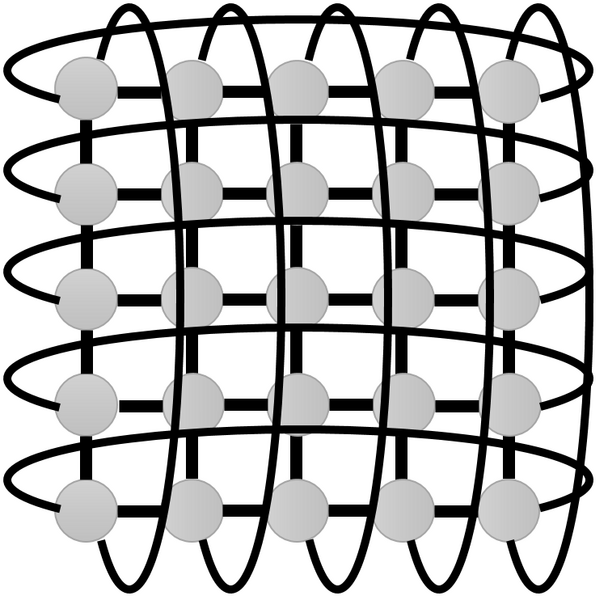
\includegraphics[width=0.5\textwidth]{immagini/torus_graph.png}
    \caption{esempio di torus graph \cite{torusgraph}}
    \label{fig:torus_graph}
\end{figure}

Tuttavia, le opzioni messe a disposizione dall'applicazione permettono una certa libertà di movimento,
per esempio avendo una configurazione come quella riportata in figura \ref{fig:custom_graph_example},
una volta analizzati i dati tramite l'analizzatore e forniti come imput al visualizzatore, potremmo ottenere
un risultato in cui i nodi nella matrice che abbiano un valore pari a zero, non vengano
collegati:
\begin{figure}[h]
    \centering
    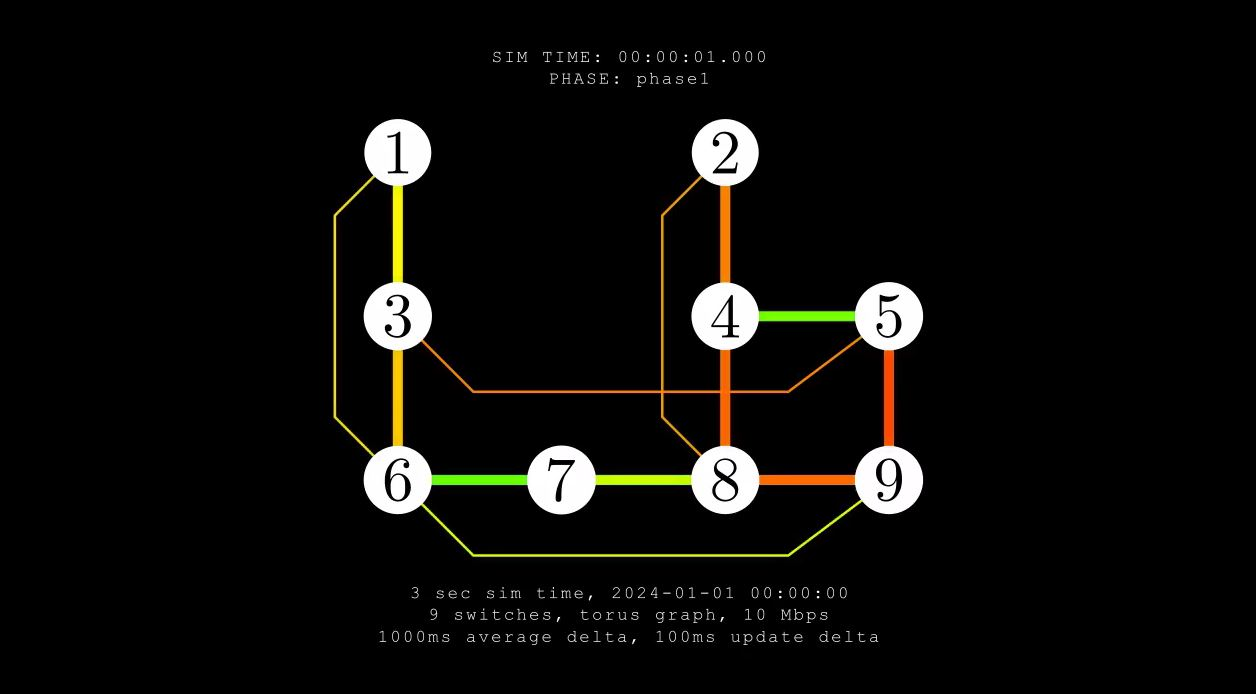
\includegraphics[width=0.8\textwidth]{immagini/only_links.JPG}
    \caption{risultato grafico del visualizzatore per un custom graph file}
    \label{fig:hybrid_custom_torus}
\end{figure}

L'ultima possibilità di personalizzazione consiste nel poter personalizzare la matrice coordinates come si preferisce, seguendo sempre la regola
che laddove c'è un valore numerico, esso sarà un nodo, mentre laddove ci sarà uno zero verrà inteso come spazio vuoto. Quindi se si vuole rappresentare
un grafico che non sia di tipo mesh o torus, bisogna specificare nel campo graphType il valore "graph", mostriamo un esempio:

{\scriptsize % Cambia la dimensione del testo per il blocco lstlisting
\begin{lstlisting}[caption={esempio di custom graph file, graphType posto al valore graph}]
    ---
    data:
      graphType: graph
      coordinates:
        - [0, 0, 0, 0, 1, 0, 0, 0, 0]
        - [0, 0, 2, 0, 0, 0, 3, 0, 0]
        - [0, 4, 0, 5, 0, 6, 0, 7, 0]
      linkCap: 10
      switches:
        1:
          ip: "123.123.123.0"
          switchName: A
        2:
          ip: "123.123.123.1"
          switchName: B
        3:
          ip: "123.123.123.2"
          switchName: C
        4:
          ip: "123.123.123.3"
          switchName: D
        5:
          ip: "123.123.123.4"
          switchName: E
        6:
          ip: "123.123.123.5"
          switchName: F
        7:
          ip: "123.123.123.6"
          switchName: G
      links:
        - [1, 2]
        - [1, 3]
        - [2, 4]
        - [2, 5]
        - [3, 6]
        - [3, 7]
      phases:
        2024-01-01 00:00:01: "phase1"
        2024-01-01 00:00:02: "phase2"
\end{lstlisting}
}

Come possiamo intuire osservando i valori nel campo coordinates, l'esempio ricrea la struttura di un albero, i links sono appunto specificati 
nel campo link e una volta generato il traffico con il generatore, analizzato e dato come input 
al visualizzatore otteniamo un risultato come in figura \ref{fig:tree_custom}.
\newline
\begin{figure}[h]
    \centering
    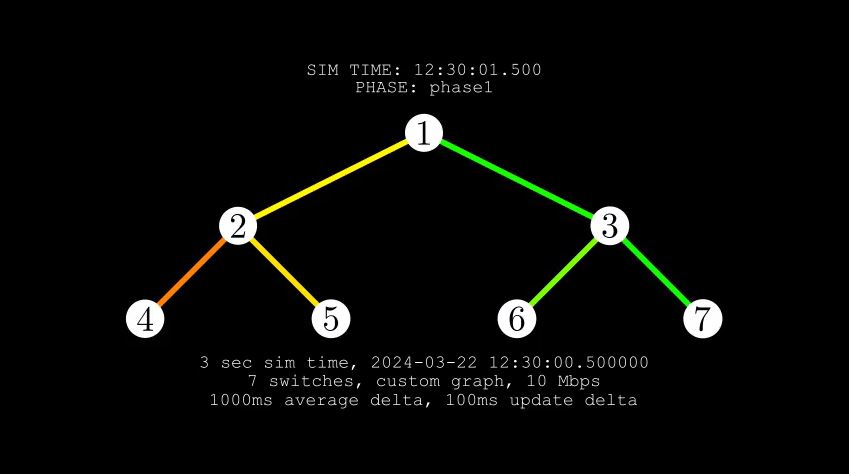
\includegraphics[width=0.8\textwidth]{immagini/free_graph.JPG}
    \caption{risultato grafico del visualizzatore per un custom graph file in modalità "graph"}
    \label{fig:tree_custom}
\end{figure}
Vien da sè che si ottiene così una certa libertà di espressione bidimensionale, con la quale l'utente può scegliere
la rappresentazione che più si addice alla rete che si vuole realizzare.

\section{Esecuzione del generatore}
Il generatore può essere pensato come suddiviso in sezioni logiche per quanto riguarda la stesura del codice nello script; la prima riguarda la fase
di interazione con l'utente, il codice  strutturato in una serie di richieste per l'utente e controlli sul corretto inserimento dei dati, successivamente
vi è la parte di caricamento del file contentente i parametri di rete \ref{codice:sim_setup_example}, segue la creazione dei links, la generazione del traffico
creando tutti i pacchetti, si creano le informazioni inerenti agli switch e il tutto viene memorizzato sui files. Vedremo più in dettaglio questi
aspetti, a livello di codice, nel capitolo dedicato allo studio della complessità computazionale e prestazioni, mentre in questo capitolo ci focalizzeremo
sulla descrizione su come viene generato il tutto.
Descriveremo ora il funzionamento dell'esecuzione vera e propria dello script relativo alla generazione del traffico e dei files che produrrà.
All'avvio l'utente sarà chiamato a scegliere tra due modalità, come accennato precedentemente, auto e user; scegliendo auto verrà chiesto all'utente
di scegliere il numero di switch che si vuole attribuire alla rete, da un minimo di due a un massimo di mille. Questo intervallo numerico nasce per
poter rappresentare una rete in un generico data center, il quale generalmente ospita fino a un migliaio di switch. Ciò non toglie che,
in un ottica futura di espansione del software, questo range non possa essere espanso con le dovute modifiche. Successivamente alla scelta nel numero
di switch l'utente sarà chiamato a scegliere la tipologia di rete potendo scegliere tra i valori "c" (completo), "m" (mesh) e "t" (torus). Per 
grafo completo
si intende quando un nodo è collegato a tutti i nodi rimanenti, è il grafo computazionalmente parlando più oneroso da ricreare per via 
della grande crescita
del numero di archi da rappresentare al crescere dei nodi. Avendo infatti \(n\) nodi avremo un numero di link \(l\) pari a:
\begin{equation}
    l = \frac{n(n-1)}{2}
    \label{eq:link_number}
\end{equation}
Ogni nodo è collegato a tutti gli altri meno se stesso, \(n(n-1)\), e si divide per due perchè gli archi non vanno contati due volte. Si parla quindi di una crescita esponenziale al variare del numero di nodi.
Per grafo mesh si è inteso una rappresentazione in cui ogni nodo ha quattro nodi adiacenti, fatta eccezione di coloro che risiedono alle estremità, come
raffigurato nell'esempio in figura creato dal visualizzatore \ref{fig:mesh_example}.
\begin{figure}[h]
    \centering
    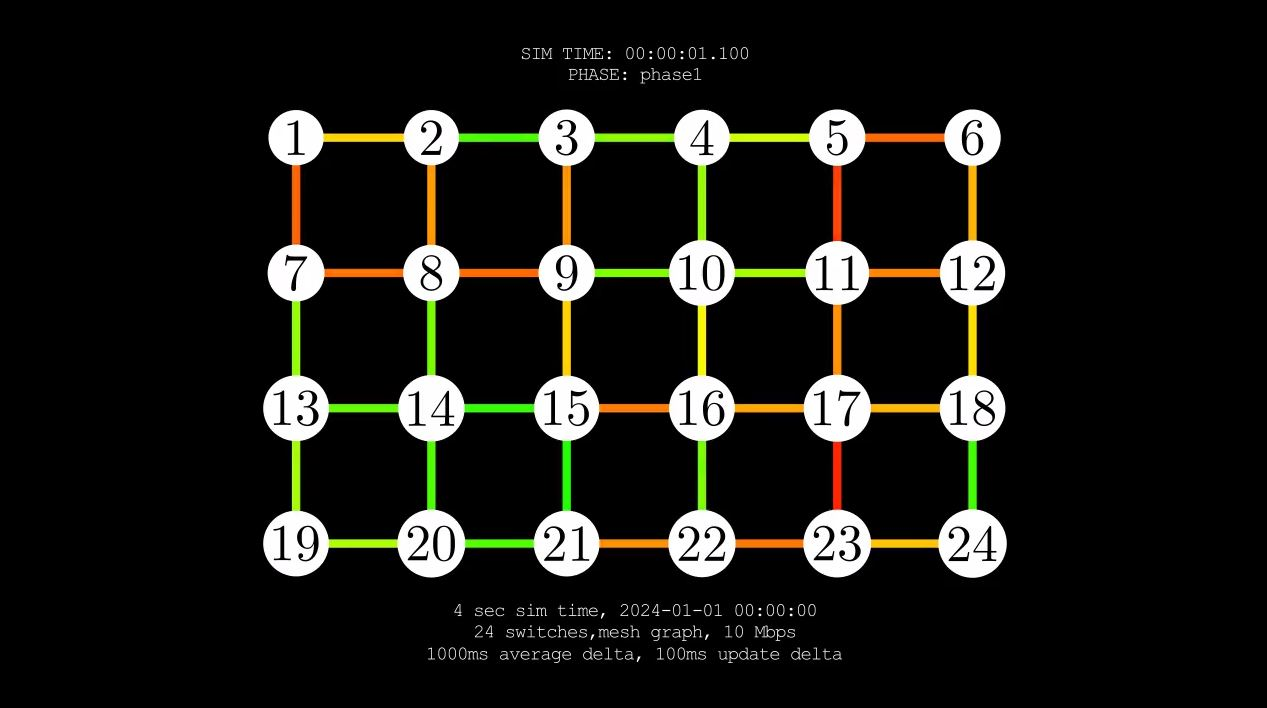
\includegraphics[width=0.8\textwidth]{immagini/mesh_example.jpg}
    \caption{risultato grafico del visualizzatore per un auto mesh graph}
    \label{fig:mesh_example}
\end{figure}
Nel caso della scelta di un grafico torus, il visualizzatore provvederà a disegnare la struttura come mostrata in figura \ref{fig:torus_graph}.
La scelta successiva in cui l'utente sarà invitato a fornire, riguarda la capacità che si vuole associare ai link appartenenti alla rete, potendo
scegliere tra i valori 10, 100 e 1000 e vengono intese come grandezze espresse in megabytes (MB).
Una volta inseriti questi parametri il generatore provvederà a creare la configurazione di rete e il rispettivo traffico, memorizzando i dati rispettivamente
nei files network.yaml e packets.json/yaml.
Scegliendo la modalità user non viene richiesto alcun dato via prompt, questo perchè, come descritto in precedenza, tutti i dati di cui ha bisogno
il generatore devono essere presenti nel file custom\_graph.yaml \ref{fig:custom_graph_example}. Un diagramma che illustra le fasi e le
 scelte cui è possibile fare
è rappresentato in figura \ref{fig:diagramma_generatore}.   
\begin{figure}[h]
    \centering
    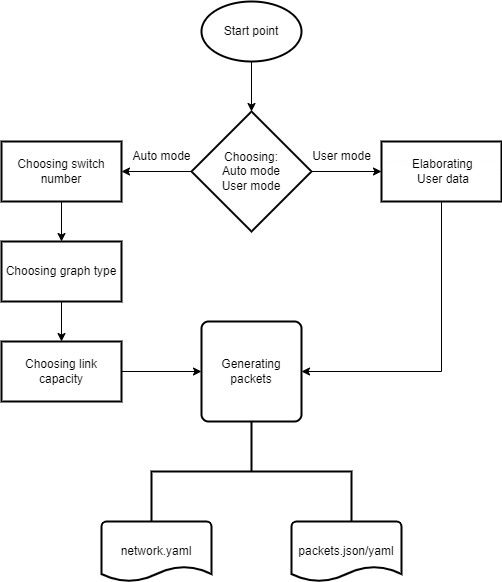
\includegraphics[width=0.40\textwidth]{immagini/diagramma_selezioni_config_gen.jpg}
    \caption{diagramma di flusso di esecuzione del generatore}
    \label{fig:diagramma_generatore}
\end{figure}


Il generatore si serve di una serie di funzioni di utilità per creare le strutture in base alle scelte dell'utente. 
Tutte le tipologie di rappresentazioni avvengono seguendo una logica di distribuzione dei nodi in forma matriciale, fatta eccezione della tipologia di
grafo completo (spiegheremo nella parte dedicata al visualizzatore il perchè), come descritto in dettaglio nel prossimo paragrafo.


\section{Creazione dei links e nodi}
Dopo aver effettuato le scelte via prompt e dopo che il programma ha caricato i parametri dal file sim\_setup.yaml 
avviene la creazione dei link e dei nodi. Per i link viene creata una struttura che consiste in un dizionario in cui ogni chiave sarà associata
ai parametri del link con un identificativo come chiave:

{\scriptsize % Cambia la dimensione del testo per il blocco lstlisting
\begin{lstlisting}[language=Python, caption={esempio di rappresentazione di un link}, label={codice:links_key_value}]
    {
        "endpoints": sorted((switch_a, switch_b)),
        "capacity": link_cap,
        "trafficPerc": 0
    }
\end{lstlisting}
}
Il campo enpoints rappresenta i nodi che il link collega, capacity è la capcità del link e trafficPerc è la percentuale di traffico del link.
Le percentuali di traffico del link sono pensate per variare ogni secondo di generazione e servono solo ai fini della creazione della quantità di traffico, questo specifico campo non sarà riportato nel network.yaml
pochè è un dato che non servirà più, di fatti la struttura che rappresenta i link verrà memorizzata come una lista di dizionari come segue:


{\scriptsize % Cambia la dimensione del testo per il blocco lstlisting
\begin{lstlisting}[caption={esempio di struttura finale dei links}, label={codice:links_structure}]
  - capacity: 10
    endpoints:
    - 1
    - 2
  - capacity: 10
    endpoints:
    - 2
    - 3
  - capacity: 10
    endpoints:
    - 1
    - 4
  - capacity: 10
    endpoints:
    - 4
    - 5
\end{lstlisting}
}

Il campo \(capacity\) identifica la capacità del link espressa in MB, mentre \(endpoints\) è una lista di due identificatori numerici compresi tra
2 e 1000 che rappresentano i nodi che li collega.
Ci sono diverse configuazioni che lo script sarà tenuto a considerare in base alle scelte dell'utente, possiamo individuarle in:

\begin{itemize}
    \item \textbf{Modalità auto:} ci sono 3 configurazioni possibili, complete graph, mesh e torus.
    \begin{itemize}
        \item \textbf{Complete graph:} i links vengono in modo tale che ogni nodo sia collegato a tutti i nodi rimanenti. Non c'è un riferimento esplicito al posizionamento poichè, come vedremo successivamente, sarà compito del visualizzatore grafico disporre i nodi nello spazio.
        \item \textbf{Mesh graph: } i links vengono creati in modo tale che ogni nodo abbia 4 nodi adiacenti rispetto a una distribuzione spaziale su matrice rettangolare, a eccezione dei nodi che risiedono alle estremità.
        \item \textbf{Torus graph: } i links vengono creati in modo da replicare il più possibile la struttura di un torus graph completo, come mostrato in fig. \ref{fig:torus_graph} utilizzando lo stesso sistema di disposizione usato per il mesh graph basato su matrice rettandolare.
        Qualora il numero di nodi scelto non riesca a riempire la matrice, l'algoritmo non creerà i link di nodi che non risultino essere alle estremità.
    \end{itemize} 
    \item \textbf{Modalità user:} i links vengono semplicemente caricati dal file e copiati nella struttura. Nel caso in cui i link non siano specificati nel custom file allora vengono generati.
\end{itemize}
In questa fase i nodi (ovvero gli endpoints) sono definiti tramite il campo \(enpoints\) dei vari links, solo successivamente verrà aggiunto l'indirizzo di ciascun endpoint, un suo nome e l'ID.
Nel caso di modalità auto vengono creati indirizzi automaticamente a partire da \(10.0.0.1\), l'identificativo è un valore numerico crescente a partire da 1 e il nome è semplicemente la composizione
della parola \(switch\) seguita dall' ID, come ad esempio \(switch1\).
Nel caso di modalità user tutte le informazioni inerenti agli switch saranno copiate nella struttura così come sono memorizzate nel file custom\_graph.yaml

\section{Distribuzione dei nodi: aspect ratio}
Come accennato precedentemente, la distribuzione dei nodi è pensata per essere disegnata in forma matriciale, questo segue una precisa scelta di design e riguarda
l'aspect ratio adotatto per disegnare al meglio gli elementi su schermo tramite la libreria Manim, la quale produce video in 16:9, quindi è sorta l'esigenza
di sfruttare al massimo questo formato visivo per poter inserire nel modo più coerente e ottimizzato possibile i vari elementi della rete.
La soluzione adottata è stata quella di pensare al numero di nodi come un'area di un quadrato (matrice quadrata) e successivamente trovare l'area equivalente 
di un rettangolo (matrice rettangolare) considerando un
aspetc ratio di 16:9. Consideriamo il numero di nodi \(A\) come l'area del quadrato e con \(n\) un suo lato \(n = \sqrt{A}\).
Denotiamo con $l$ la lunghezza e con $h$ l'altezza del rettangolo. La condizione di proporzione si può esprimere come
\[
\frac{l}{h} = \frac{16}{9}.
\]
Dato che l'area del rettangolo deve essere uguale a quella del quadrato, abbiamo che
\[
l \cdot h = n^2.
\]
Utilizzando la proporzione, possiamo esprimere $l$ in termini di $h$ come
\[
l = \frac{16}{9}h.
\]
Sostituendo questa espressione nell'equazione dell'area, otteniamo
\[
\frac{16}{9}h \cdot h = n^2,
\]
che si semplifica in
\[
\frac{16}{9}h^2 = n^2.
\]
Da qui, isoliamo $h$ ottenendo
\[
h^2 = \frac{9}{16}n^2 \quad \Longrightarrow \quad h = n \cdot \frac{3}{4}.
\]
Risostituendo il valore di $h$ nell'espressione di $l$, abbiamo
\[
l = \frac{16}{9} \cdot n \cdot \frac{3}{4} = n \cdot \frac{4}{3}.
\]
Abbiamo ottenuto la base \(l\), corrispondente al numero di colonne della matrice, e l'altezza \(h\), corrispondente al numero
di righe, del rettangolo in 16:9. Tuttavia c'è l'esigenza di rappresentare numeri interi poichè la radice dell'area \(A\) può non essere un numero intero e di conseguenza anche \(l\) e \(h\).
Per ovviare al problema si è deciso di arrotondare \(l\) e \(h\) all'intero superiore, così facendo, qualora si avesse
il lato \(s\) avente parte decimale, sarà sempre verificato:
\begin{equation}
    (l+1)(h+1)>lh
\end{equation}
riuscendo a contenere l'area e rimanendo in proporzione.

\section{Generazione del traffico}
Successivamente alla creazione dei link e dei nodi vi è la generazione del traffico, ovvero la creazione di tutti i pacchetti che vengono
creati. Descriveremo ora il criterio di creazione del traffico; l'idea è quella di iterare su frazioni di tempo cui l'unità temporale è definita
 dal campo creationDelta (tutti i campi che citeremo provengono dal file setup sim\_setup.yaml). L'algoritmo cicla per ogni frazione di 
 tempo per la durata della generazione, definita nel campo
 simTime e per ciascuna calcola un quantitativo di pacchetti, proporzionale alla 
percentuale di traffico, per ogni link presente nella rete. Ogni secondo trascorso viene cambiata la percentuale di traffico di ogni link secondo
la scelta fatta nel campo trafficVariation.
Il tempo, data e ora, che definisce quando è cominciata la trasmissione lo ritroviamo nel timestamp startSimTime.
Poichè per ogni frazione il calcolo dei pacchetti può non essere preciso, ovvero può capitare che ci sia un numero con una parte decimale, l'algoritmo
provvede a recupere questa rimanenza, tramutarla in pacchetto e aggiungerla. Questo fa si di avere un'elevata approssimazione, tendente al 100\% per
quanto riguarda l'essere più fedeli possibili alle percentuali di traffico da generare.



\section{Files prodotti}
\label{sec:files_prodotti}
Una volta creati links e nodi, generato il traffico, costruito le strutture del traffico e della rete, lo script provvederà a salvare il risultato nei files descritti precedentemente.
Un esempio di file network lo ritroviamo in figura \ref*{codice:network_file_example}.
{\scriptsize % Cambia la dimensione del testo per il blocco lstlisting
\begin{lstlisting}[caption={esempio di network file}, label={codice:network_file_example}]
- - capacity: 10
    endpoints:
    - 1
    - 2
  - capacity: 10
    endpoints:
    - 1
    - 3
  - capacity: 10
    endpoints:
    - 3
    - 4
  - capacity: 10
    endpoints:
    - 2
    - 4
- - address: 10.0.0.1
    switchID: 1
    switchName: switch1
  - address: 10.0.0.2
    switchID: 2
    switchName: switch2
  - address: 10.0.0.3
    switchID: 3
    switchName: switch3
  - address: 10.0.0.4
    switchID: 4
    switchName: switch4
- averageDelta: 1000
  colorblind: 'no'
  dotsSize: fixed
  graphType: mesh
  linkCap: 10
  packetsFile: json
  simTime: 5
  startSimTime: 2024-03-22 12:30:00
  updateDelta: 100
- coordinates:
  - - 1
    - 2
  - - 3
    - 4
- 2024-03-22 12:30:01: phase1

\end{lstlisting}
}
Il file è una lista contenente tutti i valori relativi alla configurazione network, avendo i seguenti campi nell'ordine:

\begin{itemize}
    \item Una lista di links ognuno dei quali descrive la capacità e gli endpoints al quale è collegato
    \item Una lista di switch ognuno dei quali descrive l'indirizzo, il proprio identificativo e un eventuale nome associato
    \item Un oggetto rappresentante un dizionario con i parametri di rete:
    \begin{itemize}
        \item averageDelta: l'intervallo di tempo delle medie percentuali di traffico da calcolare con l'analizzatore espressi in millisecondi
        \item colorblind: yes/no, abilita nel caso di scelta "yes" una palette cromatica nel visualizzatore grafico adatta a persone affette da daltonismo
        \item dotSize: fixed/adaptive, un'opzione che rende uguale la dimensione a tutti gli elementi raffiguranti gli switch nel visualizzatore grafico (fixed), oppure che adatta la dimensione alla lunghezza dell'identificativo degli switch (adaptive)
        \item graphType: la tipologia del grafo da visualizzare (complete, mesh, torus)
        \item linkCap: valore compreso tra [10, 100, 1000]/mixed, un valore che identifica la capacità dei links qualora fossero tutti della stessa grandezza, mixed altrimenti
        \item packetsFile: json/yaml, la scelta del formato con il quale si vuole memorizzare il traffico di rete
        \item simTime: la durata complessiva delle operazioni di rete
        \item startSimTime: timestamp, data e ora nel formato YY:MM:DD HH:MM:SS dell'inizio della trasmissione del traffico
        \item updateDelta: un intervallo temporale che identifica ogni quanto la media averageDelta debba essere aggiornata
    \end{itemize}
    \item Una lista di liste che descrive la matrice del posizionamento degli switch.Nel caso di scelta di grafo completo questo campo è una lista vuota ([])
    \item Una lista di fasi temporali che descrivono specifici intervalli temporali nel formato "YY:MM:DD HH:MM:SS = descrizione fase"
\end{itemize}
Il generatore crea delle fasi descrittive ogni 10 secondi di simulazione e le memorizza come ultimo valore della lista della struttura network.
Per il file packets abbiamo invece due possibili risultati in base alla scelta fatta nel file di setup \ref{codice:sim_setup_example}, ovvero json e yaml.
Il generatore crea i pacchetti secondo l'assunzione in cui essi vengano registrati in ordine di invio, avremo quindi una struttura corrispondente
a una lista di pacchetti ordinati per timestamp di invio.
Le strutture si presentano come in figura \ref{codice:json_packets_file} per il formato json e in figura \ref{codice:yaml_packets_file} per il formato yaml.
Come vedremo nel prossimo capitolo, questi due files rappresentano l'esatto formato che riesce a leggere l'analizzatore, quindi un utente
che voglia usare l'analizzatore e il visualizzatore grafico dovrà formattare accuratamente i suoi dati come descritto.

{\scriptsize % Cambia la dimensione del testo per il blocco lstlisting
\begin{lstlisting}[caption={esempio di packets file in formato json}, label={codice:json_packets_file}]
[
    {
        "A": 1,
        "B": 2,
        "t": "2024-03-22 12:30:00",
        "d": 4000
    },
    {
        "A": 2,
        "B": 1,
        "t": "2024-03-22 12:30:00",
        "d": 4000
    },
    {
        "A": 2,
        "B": 1,
        "t": "2024-03-22 12:30:00",
        "d": 4000
    }
]
\end{lstlisting}
}

{\scriptsize % Cambia la dimensione del testo per il blocco lstlisting
\begin{lstlisting}[caption={esempio di packets file in formato yaml}, label={codice:yaml_packets_file}]
  - A: 1
    B: 2
    d: 4000
    t: &id001 2024-03-22 12:30:00
  - A: 1
    B: 2
    d: 4000
    t: *id001
  - A: 1
    B: 2
    d: 4000
    t: *id001
\end{lstlisting}
}

In cui in entrambi i casi abbiamo i seguenti campi:
\begin{itemize}
    \item A: l'endpoint di partenza del pacchetto
    \item B: l'endpoint di arrivo del pacchetto
    \item d: la dimensione del payload del pacchetto espresso in Bytes
    \item t: il timestamp rappresentante la data e l'ora di invio del pacchetto
\end{itemize}
La scelta di usare un solo carattere per descrivere i vari campi può sembrare in contrasto con la volontà di rendere leggibile il tutto,
ma c'è una valida motivazione dietro. Il risparmio di caratteri, in files che sono potenzialmente molto grandi, è un aspetto cruciale sia per quanto
riguarda l'occupazione di memoria, sia per motivi di efficienza. Consideriamo una rappresentazione di un pacchetto più descrittivo come in figura \ref{codice:long_description_packet}:

{\scriptsize % Cambia la dimensione del testo per il blocco lstlisting
\begin{lstlisting}[caption={rappresentazione di un pacchetto con descrizione completa}, label={codice:long_description_packet}]
{
    "endpointA": 1,
    "endpointB": 2,
    "timestamp": "2024-03-22 12:30:00",
    "dimension": 1518
}
\end{lstlisting}
}

Avremmo così 37 bytes necessari per i nomi dei campi contro i 4 per la rappresentazione di un pacchetto descritta precedentemente, avendo uno scarto di
33 bytes per pacchetto. Questa quantità, moltiplicata la grande quantità di pacchetti da rappresentare, può pesare non poco.
Indipendentemente dal numero di bytes necessari a rappresentare un pacchetto in forma minimale, possiamo fare una stima di quanto sarebbe più grande
un file packets avendo descrizioni di nomi più lunghi; supponiamo di avere un grafo completo costituito da 5 switch collegati tra loro con switch
aventi capienza 1 Gbps (gigabit), il numero dei link, per l'equazione in fig. \ref{eq:link_number}, risulta essere pari a 10. Supponiamo che tutta la rete
stia trasmettendo al 50\% della sua capacità trasmissiva per tutta la durata dell'attività di rete. Considerando una dimensione \(d\) di payload pari 
a 1518 Bytes uguale per tutti i pacchetti trasmessi,
definiamo come \(pps\) i pacchetti al secondo, da cui, per un link in un dato secondo avremo:
\begin{align*}
    \text{1 Gbps} &= 10^9 \text{ bit}\\
    \text{1 GBps} &= \frac{10^9}{8} = 125,000,000 \text{ bytes} && \text{(1 byte = 8 bit)} \\
    \text{50\% capacity} &= \frac{125,000,000}{2} = 65,500,000 \text{ bytes}\\
    \text{d} &= 1518 \text{ bytes} \\
    \text{pps} &= \frac{65,500,000 \text{ bytes}}{d}\approx 41172.59\\
    \text{bytes di differenza} &= 41172.59 \times 33 \approx 1.35 \text{ MBytes}
\end{align*}
Ciò significa che per ogni secondo di traffico avremmo \(1.35 \text{ MB} \times 10\text{ links} = 13.5 \text{MB}\) in più, 
 in 100 secondi di traffico avremmo 1350 Mbytes, cioè 1.35 GBytes in più per una rete avente soltanto 10 links, quindi con la scelta di rendere
  mono carattere le descrizioni
 si ha un notevole risparmio in termini di data storage. Chiaramente in ottica di espansione futura del progetto, avendo strutture più complesse
 per i pacchetti, potrebbe essere necessario avere elementi maggiormente descrittivi, tuttavia ciò non toglie che una certa cura nella scelta di una 
 descrizione minimale non possa essere comunque adottata in via preferenziale.


 \section{Aspetti realizzativi scartati: yaml flow e block style}
 Un approccio inizialmente realizzato e poi scartato, è stato quello di poter dare la possibilità di scegliere la modalità di salvataggio del file packets.yaml.
La libreria PyYAML permette di salvare un file yaml secondo due modalità; la prima è definita block style e l'altra flow style.
Di default, PyYAML sceglie lo stile di una collection a seconda che abbia a sua volta collection nidificate. Qualora ci fossero collection nidificate
verrà assegnato lo stile block, il quale è il formato come lo abbiamo già visto in figura \ref{codice:yaml_packets_file}, altrimenti verrà assegnato
lo stile flow che corrisponde al codice in figura.

{\scriptsize % Cambia la dimensione del testo per il blocco lstlisting
\begin{lstlisting}[caption={rappresentazione di un pacchetto con descrizione completa}, label={codice:long_description_packet}, breaklines=true]
[{A: 2, B: 1, d: 4000, t: &id001 !!timestamp '2024-03-22 12:30:00'}, {A: 1, B: 2,
    d: 4000, t: *id001}, {A: 1, B: 2, d: 4000, t: *id001}, {A: 2, B: 1, d: 4000, t: *id001},
  {A: 2, B: 1, d: 4000, t: *id001}, {A: 2, B: 1, d: 3752, t: *id001}, {A: 1, B: 2,
    d: 4000, t: &id002 !!timestamp '2024-03-22 12:30:00.100000'}, {A: 2, B: 1, d: 4000,
    t: *id002}, {A: 1, B: 2, d: 4000, t: *id002}, {A: 1, B: 2, d: 4000, t: *id002},
  {A: 2, B: 1, d: 4000, t: *id002}, {A: 2, B: 1, d: 3752, t: *id002}, {A: 1, B: 2,
    d: 4000, t: &id003 !!timestamp '2024-03-22 12:30:00.200000'}, {A: 2, B: 1, d: 4000,
    t: *id003}, {A: 2, B: 1, d: 4000, t: *id003}, {A: 1, B: 2, d: 4000, t: *id003},
\end{lstlisting}
}
Inizialmente si era provato a dare la possibilità di scegliere, tramite file sim\_setup, 
tra il formato block e flow poichè in fase di test
si è visto che l'opzione flow riduce ulteriormente la dimensione del file packets.yaml. Tuttavia i test hanno dimostrato che le differenze delle grandezze
dei files e i tempi necessari a realizzarli non erano così diversi tra loro, quindi si è deciso di scartare del tutto l'opzione. Possiamo vedere
il risultato del test sulle dimensioni dei files in figura \ref{fig:yaml_block_flow_dim}, dove troviamo sull'asse delle ascisse il numero di switch per test, mentre
sull'asse delle ordinate abbiamo la variabile che esprime i megabytes, questo perchè essa è la variabile dipendente, ovvero i megabytes dipendono dal numero di switch
che viene scelto. Il grafico relativo ai tempi di scrittura/lettura lo troviamo in 
figura \ref{fig:yaml_block_flow_wr}, in questo caso abbiamo sull'asse delle ascisse sempre il numero di switch per test, mentre sull'asse delle ordinate
il tempo (in secondi) necessario per le scritture e letture, poichè il tempo di computazione dipende dal numero di switch scelto. Possiamo notare dai grafici che il risparmio di bytes è di circa 4 MB per il test effettuato su 10 switch, mentre
i tempi di esecuzione, sia di scrittura che di lettura, sono praticamente sovrapponibili, infatti l'operazione di scrittura per block e flow style è identico, mentre lievemente
più performante è il block style in lettura.

\begin{figure}[h]
    \centering
    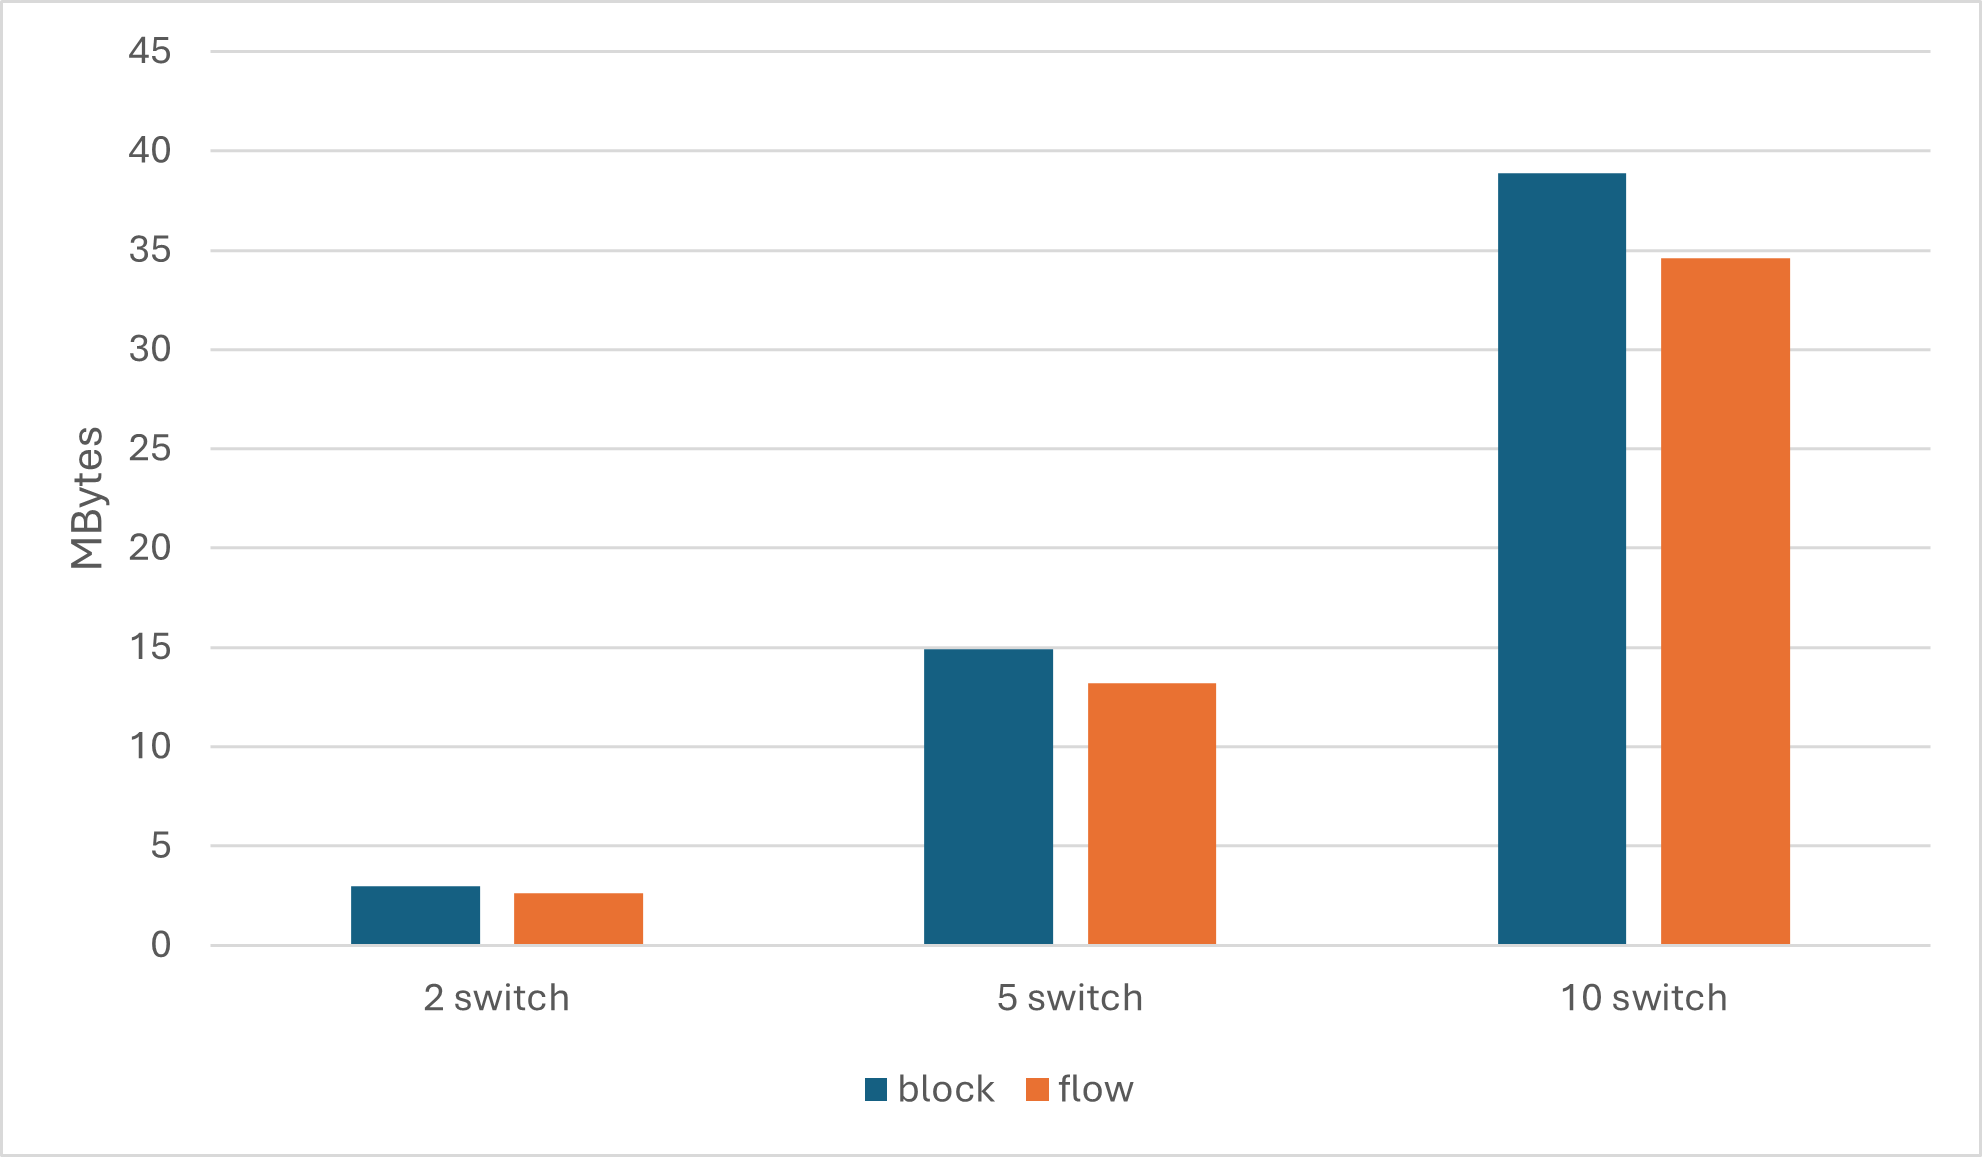
\includegraphics[width=1\textwidth]{immagini/yaml_block_flow_dim.png}
    \caption{test yaml block/flow style, dimensione files}
    \label{fig:yaml_block_flow_dim}
\end{figure}

\begin{figure}[h]
    \centering
    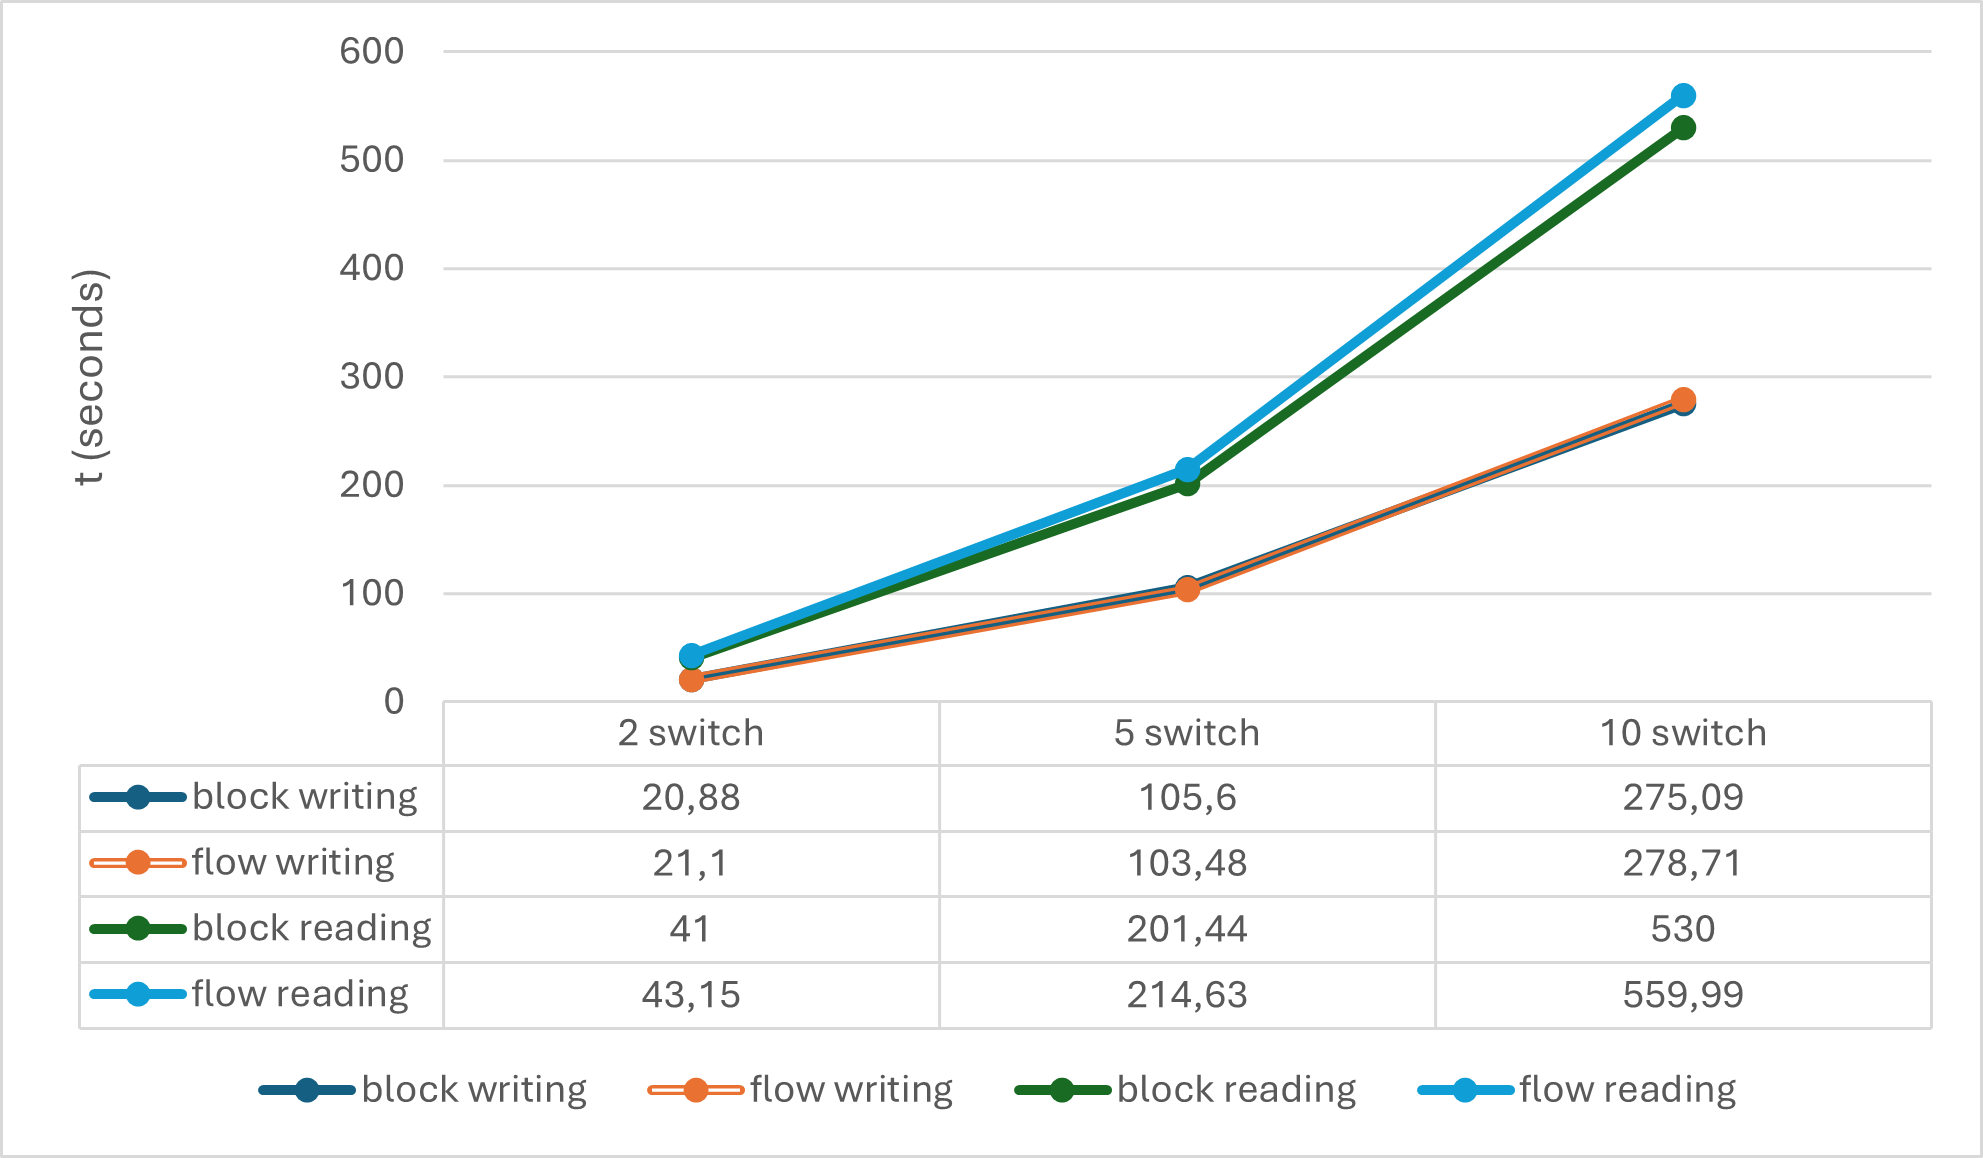
\includegraphics[width=1\textwidth]{immagini/yaml_block_flow_wr.png}
    \caption{test yaml block/flow style, tempi di scrittura e lettura}
    \label{fig:yaml_block_flow_wr}
\end{figure}




\chapter{Analizzatore di traffico}
L'analizzatore di traffico è la seconda anima del progetto essendo la parte che analizza il traffico calcolando le medie percentuali e che produce
un file, analyzed\_data.yaml, che conterrà sia le informazioni di rete come links, switches e parametri di rete, sia le registrazioni del traffico percentuale
di ogni link. Per poter operare, l'analizzatore ha bisogno dei due files, network.yaml e packets.yaml, creati dal generatore o che siano
creati e formattati dall'utente. Abbiamo descritto in dettaglio la composizione dei files nella sezione \ref{sec:files_prodotti}.
L'esecuzione dello script parte in primo luogo caricando i files richiesti e creando le strutture necessarie al calcolo delle medie, dopodichè
avviene il calcolo vero e proprio, viene creata la struttura che servirà come input del visualizzatore grafico e infine viene creato il file
analyzed\_data.yaml con tale struttura.
Poichè per motivi di efficienza si è scelto di strutturare i link come una lista nel file network.yaml e non come dizionario (in cui ogni link avrebbe avuto un identificativo come chiave), si è presentato il problema dell'identificazione dei link.
I link in fin dei conti possono essere identificati dai propri endpoints (il grafo viene inteso in modo tale che ci sia un unico link tra due endpoints), ovvero una coppia di nodi,
nel nostro caso, una coppia di switch. Tuttavia la sfida che si è presentata è rappresentata dal fatto che se è vero quindi che un link è identificato
da due endpoints, a e b, è vero anche che in questo caso l'ordinamento degli endpoints non deve essere rilevante. Abbiamo infatti pacchetti
che vengono inviati sia da a per poi arrivare a b, sia da b verso a. Questo è un problema poichè stiamo cercando di identificare un link ma abbiamo
due coppie, \((a, b)\) e \((b, a)\) che sì sono ugualmente valide ma rappresentano anche due coppie distinte, il che contrasta con il concetto di identificatore. 
L'ideale sarebbe usare il tipo set, ovvero il concetto di insieme 
come collezione non ordinata in cui due insiemi \(\{b, b\}, \{b, a\}\) sono considerati uguali in termini di contenuto. Sembrerebbe un problema risolto, ma non è così, il perchè risiede
nel fatto che i set in Python sono mutabili: il contenuto può essere modificato utilizzando metodi come add() e remove(). 
Poiché set è mutabile, non ha valore hash \cite{pythonGlossaryHashable} e non può essere utilizzato come chiave del dizionario \cite{pythonStdTypesMapping}.
Il tipo di dato che fa al caso nostro è quindi il frozenset, un set che è immutabile e hashable, quindi utilizzabile come chiave di un dizionario.
Nell'analizzatore l'identificazione dei link è molto importante, perchè nel momento in cui si va a scorrere la lista di tutti i pacchetti registrati,
vi è il bisogno di identificare il link per potergli attribuire le varie medie da calcolare. Viene quindi creata una struttura ausiliaria in cui
la lista di link presente nel file network.yaml viene tramutata in un dizionario avente come chiavi dei frozenset con gli endpoints e, come valori associati,
una serie di variabili atte a mantenere le somme dei pacchetti che man mano verrano scanditi.
Segue la scansione dei pacchetti in cui, per ogni unità frazionaria di tempo dettata dal campo updateDelta presente in network.yaml, vengono sommati tutti i bytes di tutti i pacchetti
e attribuiti ai link corrispettivi.
Una volta finita la scansione, la struttura ausiliaria viene scandita per ricavare le medie percentuali delle varie somme calcolate dal passaggio precedente e viene
creata la struttura che verrà memorizzata in analyzed\_data.yaml. La struttura memorizzata è raffigurata in figura \ref{codice:analyzed_data_structure}.

{\scriptsize % Cambia la dimensione del testo per il blocco lstlisting
\begin{lstlisting}[caption={rappresentazione della struttura analyzed\_data}, label={codice:analyzed_data_structure}]
{
  - averageDelta: 1000
    simStartTime: 2024-03-22 12:30:00
    simTime: 2
    updateDelta: 100
  - - endpoints:
      - 1
      - 2
      traffic:
      - 59.0
      - 53.5
      - 48.0
      - 42.5
      - 37.0
      - 31.5
      - 26.0
      - 20.5
      - 15.0
      - 9.5
      - 4.0
    - endpoints:
      - 1
      - 3
      traffic:
      - 33.0
      - 38.8
      - 44.6
      - 50.4
      - 56.2
      - 62.0
      - 67.8
      - 73.6
      - 79.4
      - 85.2
      - 91.0
}
\end{lstlisting}
}

La struttura consiste in una lista di due elementi, il primo è un dizionario rappresentate 
i parametri di rete necessari al visualizzatore grafico, il
secondo è una lista di dizionari rappresentati i link, definiti dal campo enpoints, e le loro medie percentuali memorizzate nel campo traffic.
L'unico campo che non abbiamo ancora incontrato finora è traffic, esso rappresenta le medie percentuali di tempo averageDelta, calcolate ogni updateDelta millisecondi.
Nell esempio in figura \ref{codice:analyzed_data_structure} abbiamo che le medie vengono calcolate quindi in intervalli di 1000 ms (millisecondi), aggiornati ogni
100 ms. Prendiamo ad esempio il primo link identificato dalla coppia di endpoints \((1, 2)\), i suoi valori del campo traffic sono associati ai seguenti tempi:
\newline

{\scriptsize % Cambia la dimensione del testo per il blocco lstlisting
\begin{lstlisting}[caption={timestamps e medie percentuali calcolate dall'analizzatore}, label={codice:analyzed_data_structure}]

    2024-03-22 12:30:01 - 59
    2024-03-22 12:30:01.100000 - 53,5
    2024-03-22 12:30:01.200000 - 48
    2024-03-22 12:30:01.300000 - 42,5
    2024-03-22 12:30:01.400000 - 37
    2024-03-22 12:30:01.500000 - 31,5
    2024-03-22 12:30:01.600000 - 26
    2024-03-22 12:30:01.700000 - 20,5
    2024-03-22 12:30:01.800000 - 15
    2024-03-22 12:30:01.900000 - 9,5
    2024-03-22 12:30:02 - 4

\end{lstlisting}
}
I timestamps sono espressi nel formato YY:MM:DD HH:MM:SS.Microseconds, questo per via dell'impiego dell'oggetto timedelta \cite{pythonDatetimeTimedelta} che converte un millisecondo in 1000 microsecondi e con cui è possibile effettuare
operazioni aritmetiche di somma e differenza tra due oggetti datetime \cite{pythonDatetimeTimedelta}.
Il primo valore che abbiamo, \(59\), è quindi la media percentuale dei pacchetti inviati tra il tempo 12:30:00 e 12:30:01, il secondo valore, \(53.3\) è la media
dell'intervallo 12:30:00.100000 e 12:30:01.100000, e così via.
Il file prodotto analyzed\_data.yaml sarà l'input necessario per il visualizzatore grafico, che verrà discusso nel capitolo successivo.

\chapter{Visualizzatore grafico}
La terza anima del progetto è il visualizzatore grafico sviluppato tramite l'ausilio della libreria Manim. Andremo a descrivere il funzionamento dello script,
come è strutturato e organizzato, in seguito descriveremo le modalità grafiche dei grafi che sono possibili ottenere, inclusa la rappresentazione video
delle informazioni relative ai switch e link. Seguirà una sezione sulle scelte di design servite a curare l'aspetto visivo e infine ci sarà spazio
per l'accessibilità inclusa nel progetto che prevede un'opzione per daltonici e che consente quindi di cambiare i colori che rappresentano il traffico.

\section{Strutturazione e organizzazione del visualizzatore}
Andremo ora a descrivere come è strutturato il codice a livello logico. La prima cosa che salta all'occhio aprendo il progetto potrebbe essere la riga di codice:

{\scriptsize
\begin{lstlisting}[language=Python]
    from manim import *
\end{lstlisting}
}

Potrebbe sembrare un errore, o una scelta pigra per velocizzare le importazioni delle sezioni di libreria necessaria, ma in realtà questo è proprio
l'uso raccomandato dalla documentazione ufficiale di utilizzare Manim \cite{ManimDocs}.
Una volta avviato lo script verranno caricati i files analyzed\_data.yaml e network.yaml, successivamente verranno impostati i colori del traffico in base
alla scelta fatta nel campo colorblind all'interno del file network, dopodichè possiamo pensare al resto dello script come un bivio in cui ci sono le due funzioni principali;
la funzione che renderizzerà il grafo in caso di grafo completo e la funzione che renderizzerà un grafo pensato per essere disposto
tramite matrice. La funzione relativa al grafo completo sfrutta la potenza di Manim per la disposizione dei nodi e degli archi (links), provvedendo
una disposizione automatica ed organica degli elementi e rappresenta la scelta più indicata per questo tipo di rappresentazione; per
farlo bisogna settare il campo customGraph nel file network al valore "complete" e lasciare il campo "coordinates" vuoto. Per ottenere un grafo
completo con coordinate personalizzate bisognerà assegnare a graphType il valore "graph" e specificare le coordinate nel campo "coordinates". 
Vedremo degli esempi in figura nel paragrafo successivo. Entrambe le funzioni hanno lo stesso pattern di creazione del grafico e di creazione delle animazioni;
prima si costruiscono le strutture da visualizzare, inclusi i parametri di rete da visualizzare, successivamente viene eseguito una iterazione sui timestamps ricavati
dal file analyzed\_data in cui per ogni intervallo di tempo updateTime viene presa la parcentuale corrispondente di ciascun link, 
si prendono i colori associati alle varie percentuali e si crea un'animazione di durata 1 secondo di transizione verso il colore scelto e si ripete 
fino a quando non si arriva a fine simTime.
Per dare una maggiore idea sul come vengono create le forme e le animazioni in Manim faremo una breve introduzione alla libreria.
In Manim ogni oggetto viene definito Mobject, ovvero un "Mathematical Object", e deriva dalla classe di base Mobject, cioè un oggetto che può essere visualizzato a schermo,
per esempio una forma rettangolo, una linea o un cerchio, vengono definiti tutti mobject.
La classe Scene è la tela sul quale si disegnano i mobjects, una volta istanziati essi vanno aggiunti alla Scene per poter essere visualizzati,
ciò e possibile tramite il metodo \lstinline|add()|. Prendiamo il primo esempio fornito dalla documentazione Manim:

{\scriptsize % Cambia la dimensione del testo per il blocco lstlisting
\begin{lstlisting}[language=Python, caption={un primo esempio di utilizzo di Manim \cite{ManimDocs}}, label={codice:manim_example}]
{
    from manim import *

    class CreatingMobjects(Scene):
        def construct(self):
            circle = Circle()
            self.add(circle)
            self.wait(1)
            self.remove(circle)
}
\end{lstlisting}
}

Come descrive la documentazione ufficiale, generalmente tutto il codice che descrive un video va all'interno del metodo \lstinline|construct()|
della classe \lstinline|Scene|, per poter visualizzare un mobject si chiama il metodo \lstinline|add()| della \lstinline|Scene| contenuta, in questo caso
passiamo un mobject \lstinline|circle| come parametro, aggiungendolo alla \lstinline|Scene|.
Il metodo \lstinline|wait(1)| fa passare un secondo di tempo e \lstinline|remove(circle)| lo rimuove.
Si intuisce da subito le potenzialità che offre la libreria ma sono le animazioni il cuore di Manim.
Ogni proprietà di un mobject che può essere modificata, può essere animata. Infatti ogni metodo che cambia una proprietà di un mobject può essere
usato come un'animazione tramite l'uso di \lstinline|animate()|.

{\scriptsize % Cambia la dimensione del testo per il blocco lstlisting
\begin{lstlisting}[language=Python, caption={un primo esempio di animazioni in Manim \cite{ManimDocs}}, label={codice:manim_animation_example}]
{
    from manim import *

    class AnimateExample(Scene):
        def construct(self):
            square = Square().set_fill(RED, opacity=1.0)
            self.add(square)
    
            # animate the change of color
            self.play(square.animate.set_fill(WHITE))
            self.wait(1)
    
            # animate the change of position and the rotation
            self.play(square.animate.shift(UP).rotate(PI / 3))
            self.wait(1)
}
\end{lstlisting}
}

Nel codice in fig. \ref{codice:manim_animation_example}, vediamo come impostare il colore rosso e il livello di opacità al mobject \lstinline|Square()|,
applicando poi il metodo \lstinline|square.animate.set_fill(WHITE)| viene creata l'animazione di transizione di colore da rosso a bianco.
L'animazione creata deve essere aggiunta alla \lstinline|Scene| per poterla visualizzare e lo si fa tramite \lstinline|play()|.
Questa breve introduzione a Manim ci da già l'idea della potenza che offre ponendo come unico limite la creatività dello sviluppatore.
Ritornando alla descrizione delle funzioni principali, il grafo completo, della funzione dedicata, viene creato tramite la classe
\lstinline|Graph()|, in cui due dei principali parametri richiesti sono una lista di valori che identificano i nomi dei nodi e una lista di coppie (tuple)
che descrivono gli archi (link). Chiaramente la liste degli switch e delle tuple di endpoints vengono create a monte. Per quanto riguarda
la creazione delle animazioni, il cuore risiede in questo pseudocodice:


{\scriptsize % Cambia la dimensione del testo per il blocco lstlisting
\begin{lstlisting}[language=Python, caption={creazione animazione traffico}, label={codice:traffic_animation_example}]
animations.append(grafo.edges[(A, B)].animate.set_color(traffic_color))
\end{lstlisting}
}
In questo pseudocodice abbiamo una lista di animazioni \lstinline|animations|, in cui aggiungiamo un'animazione \lstinline|animate| che interessa l'oggetto arco 
restituito da \lstinline|grafo.edges[(A, B)]| e individuato dalla coppia di endpoints (A, B). Dopodichè definiamo quale proprietà deve essere animata,
 in questo caso l'impostazione di un nuovo colore tramite \lstinline|set_color()| il quale è il colore corrispondente al timestamp correntemente analizzato.
Questa operazione viene effettuata per tutti i link per l'intervallo di tempo updateDelta, quando tutte le animazioni sono settate si usa
il metodo \lstinline|play(animation*)| per animarle tutte conteporaneamente e ciò si ripete per la durata di tempo registrato.

Per quanto riguarda la seconda funzione principale, il pattern di creazione è analogo, tuttavia è interessante descrivere il posizionamento dei nodi.

\section{Modalità grafiche}

\begin{figure}[h]
    \centering
    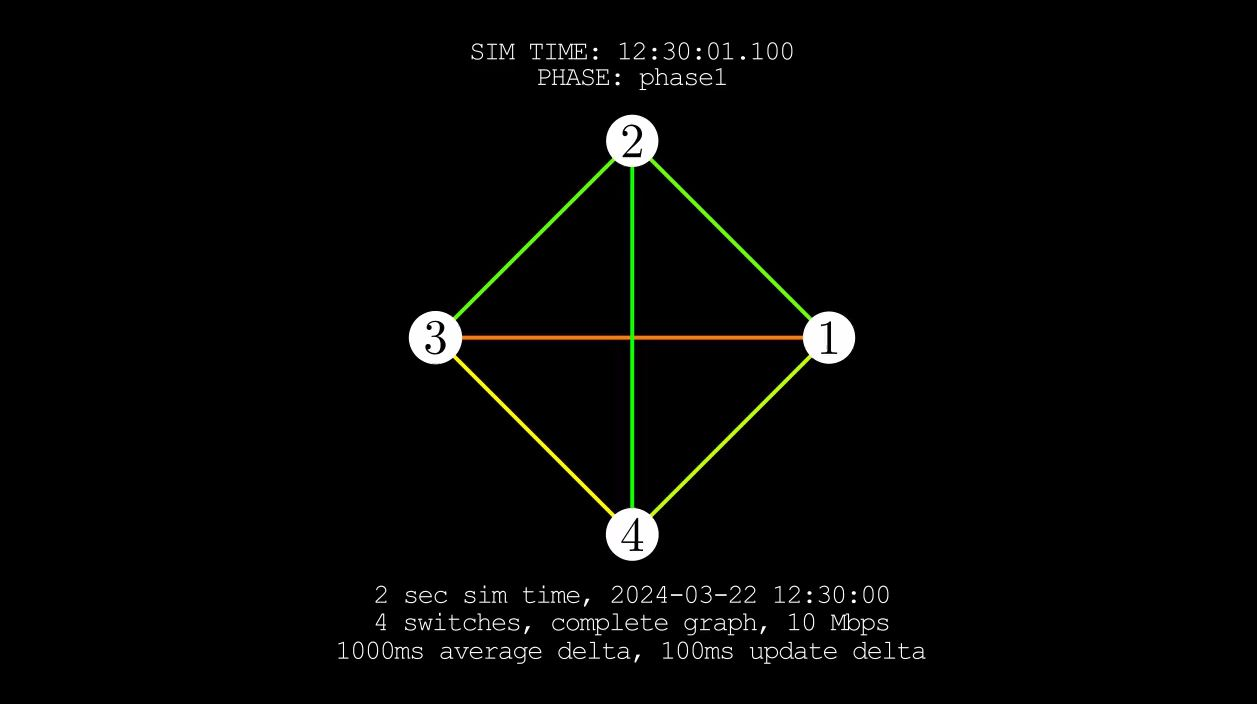
\includegraphics[width=1\textwidth]{immagini/custom_complete_autopositioning.JPG}
    \caption{visualizzazione per opzione grafo completo con disposizione automatica}
    \label{fig:custom_complete_autopositioning}
\end{figure}

\begin{figure}[h]
    \centering
    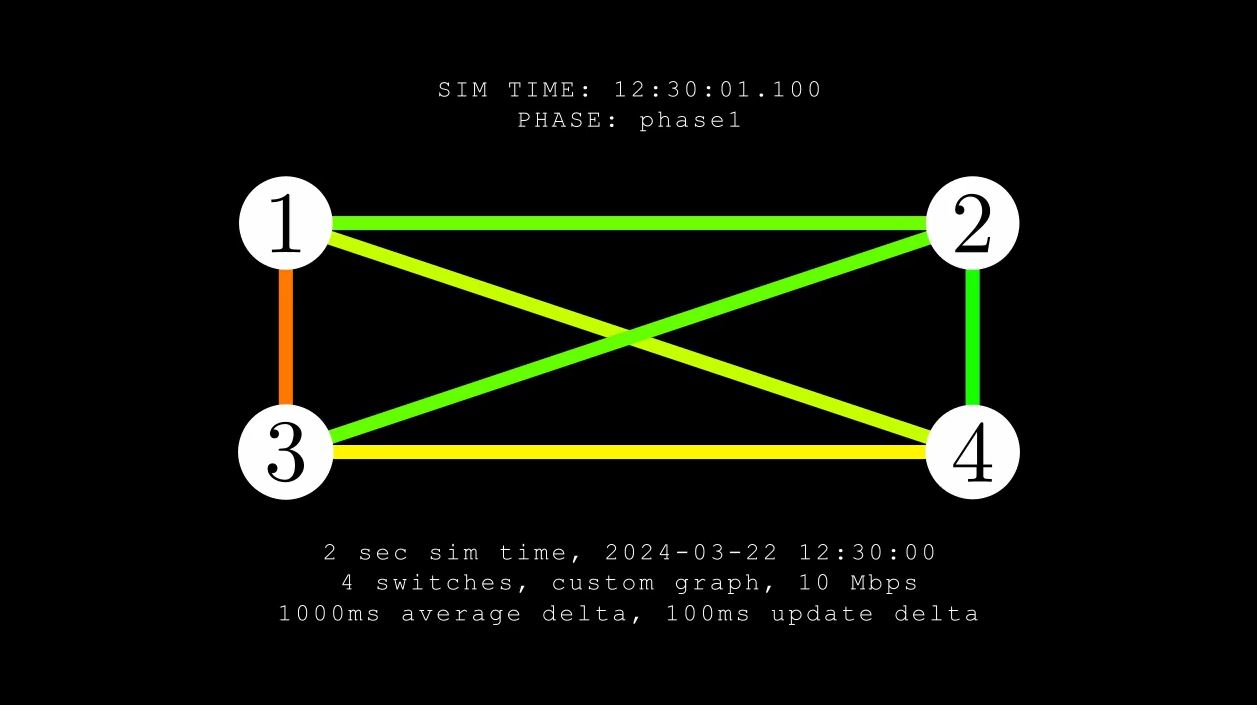
\includegraphics[width=1\textwidth]{immagini/custom_complete_manual_positioning.JPG}
    \caption{visualizzazione per opzione grafo completo con coordinate personalizzate}
    \label{fig:custom_complete_manual_positioning}
\end{figure}


\section{Design: scelte implementative}

\section{Accessibilità: modalità daltonismo}

\chapter{Prestazioni e complessità computazionale}
\section{Complessità generatore di traffico}
\section{Complessità analizzatore di traffico}
\section{Complessità visualizzatore grafico}


Per quanto riguarda la creazione automatica dei links e dei nodi
per la tipologia di grafo completo, la funzione dedicata al compito è riportata in figura \ref{codice:create_auto_complete_links}

{\scriptsize % Cambia la dimensione del testo per il blocco lstlisting
\begin{lstlisting}[language=Python, basicstyle=\ttfamily, caption={funzione per la creazione automatica di un grafo di rete completo}, label={codice:create_auto_complete_links}]
    def create_auto_complete_links(link_cap, switch_number):
    """ Create links for a complete graph 
    
    Key arguments:
    link_cap: int -- link capacity
    switch_number: int -- switch number

    Returns
    dict -- links representation
    """
    # The arcs representing the links connecting the switches (nodes)
    links = {}
    # The link ID counter
    link_id = 1

    for i in range(1, switch_number + 1):
        for p in range(i, switch_number + 1):
            if i != p:
                if link_id not in links:
                    links[link_id] = link_format(i, p, link_cap)
                    link_id += 1
    return links
\end{lstlisting}
} % Fine del gruppo che modifica la dimensione del testo

Poichè in questo caso il numero di link può essere molto elevato, consideriamo il numero di link come \(n\) essendo il ciclo for esterno condizionato
dal numero di switch. Ma se osserviamo bene notiamo che il ciclo interno parte dall'indice del ciclo for esterno. Non avremo quindi n iterazioni moltiplicato n,
ma avremo una quantità di iterazioni totali pari a:

\begin{equation}
    O\left(\sum_{i=1}^n (n-i)\right)
\end{equation}

Che andando a sviluppare risulterà essere:
\begin{align}
    O\left(\sum_{i=1}^n (n-i)\right) &= O\left(\sum_{i=1}^n n - \sum_{i=1}^n i\right) \\
    &= O\left(n\sum_{i=1}^n 1 - \sum_{i=1}^n i\right) \\
    &= O\left(n \cdot n - \frac{n(n+1)}{2}\right) \\
    &= O\left(n^2 - \frac{n^2 + n}{2}\right) \\
    &= O\left(\frac{2n^2 - n^2 - n}{2}\right) \\
    &= O\left(\frac{n^2 - n}{2}\right) \\
    &= O(n^2) \quad
    \end{align}
Poiché il termine lineare è dominato dal termine quadratico per grandi \( n \). Ciò è in linea con la grandezza intrinseca del numero di links
per un grafo completo, come visto nell'equazione \ref{eq:link_number}, per cui siamo obbligati a una complessità quadratica.
Tuttavia possiamo osservare dal calcolo:
\begin{align*}
    \sum_{i=1}^n (n-i) &= \frac{n^2 - n}{2} = \frac{n(n-1)}{2}
\end{align*}
    
IL che è esattamente l'equazione \(\frac{n(n-1)}{2}\) che determina il numero di links in un grafo completo. Con questo vogliamo dire che 
l'algoritmo performa esattamente il numero di iterazioni necessarie a creare i link ottimizzando al massimo le risorse computazionali.

\chapter{Conclusioni}
\chapter{Test}
La complessità temporale dell'algoritmo è $O(m+n)$.
\begin{equation}
    O(m+n)
\end{equation}

.. .. ..


\printbibliography

\backmatter
\cleardoublepage
\phantomsection % Give this command only if hyperref is loaded
\addcontentsline{toc}{chapter}{\bibname}
% Here put the code for the bibliography. You can use BibTeX or
% the BibLaTeX package or the simple environment thebibliography.
\end{document}